% Options for packages loaded elsewhere
% Options for packages loaded elsewhere
\PassOptionsToPackage{unicode}{hyperref}
\PassOptionsToPackage{hyphens}{url}
\PassOptionsToPackage{dvipsnames,svgnames,x11names}{xcolor}
%
\documentclass[
  11pt,
  a4paper,
  DIV=11,
  numbers=noendperiod]{scrreprt}
\usepackage{xcolor}
\usepackage[top=25mm,left=25mm,right=25mm,bottom=25mm]{geometry}
\usepackage{amsmath,amssymb}
\setcounter{secnumdepth}{5}
\usepackage{iftex}
\ifPDFTeX
  \usepackage[T1]{fontenc}
  \usepackage[utf8]{inputenc}
  \usepackage{textcomp} % provide euro and other symbols
\else % if luatex or xetex
  \usepackage{unicode-math} % this also loads fontspec
  \defaultfontfeatures{Scale=MatchLowercase}
  \defaultfontfeatures[\rmfamily]{Ligatures=TeX,Scale=1}
\fi
\usepackage{lmodern}
\ifPDFTeX\else
  % xetex/luatex font selection
\fi
% Use upquote if available, for straight quotes in verbatim environments
\IfFileExists{upquote.sty}{\usepackage{upquote}}{}
\IfFileExists{microtype.sty}{% use microtype if available
  \usepackage[]{microtype}
  \UseMicrotypeSet[protrusion]{basicmath} % disable protrusion for tt fonts
}{}
\makeatletter
\@ifundefined{KOMAClassName}{% if non-KOMA class
  \IfFileExists{parskip.sty}{%
    \usepackage{parskip}
  }{% else
    \setlength{\parindent}{0pt}
    \setlength{\parskip}{6pt plus 2pt minus 1pt}}
}{% if KOMA class
  \KOMAoptions{parskip=half}}
\makeatother
% Make \paragraph and \subparagraph free-standing
\makeatletter
\ifx\paragraph\undefined\else
  \let\oldparagraph\paragraph
  \renewcommand{\paragraph}{
    \@ifstar
      \xxxParagraphStar
      \xxxParagraphNoStar
  }
  \newcommand{\xxxParagraphStar}[1]{\oldparagraph*{#1}\mbox{}}
  \newcommand{\xxxParagraphNoStar}[1]{\oldparagraph{#1}\mbox{}}
\fi
\ifx\subparagraph\undefined\else
  \let\oldsubparagraph\subparagraph
  \renewcommand{\subparagraph}{
    \@ifstar
      \xxxSubParagraphStar
      \xxxSubParagraphNoStar
  }
  \newcommand{\xxxSubParagraphStar}[1]{\oldsubparagraph*{#1}\mbox{}}
  \newcommand{\xxxSubParagraphNoStar}[1]{\oldsubparagraph{#1}\mbox{}}
\fi
\makeatother


\usepackage{longtable,booktabs,array}
\usepackage{calc} % for calculating minipage widths
% Correct order of tables after \paragraph or \subparagraph
\usepackage{etoolbox}
\makeatletter
\patchcmd\longtable{\par}{\if@noskipsec\mbox{}\fi\par}{}{}
\makeatother
% Allow footnotes in longtable head/foot
\IfFileExists{footnotehyper.sty}{\usepackage{footnotehyper}}{\usepackage{footnote}}
\makesavenoteenv{longtable}
\usepackage{graphicx}
\makeatletter
\newsavebox\pandoc@box
\newcommand*\pandocbounded[1]{% scales image to fit in text height/width
  \sbox\pandoc@box{#1}%
  \Gscale@div\@tempa{\textheight}{\dimexpr\ht\pandoc@box+\dp\pandoc@box\relax}%
  \Gscale@div\@tempb{\linewidth}{\wd\pandoc@box}%
  \ifdim\@tempb\p@<\@tempa\p@\let\@tempa\@tempb\fi% select the smaller of both
  \ifdim\@tempa\p@<\p@\scalebox{\@tempa}{\usebox\pandoc@box}%
  \else\usebox{\pandoc@box}%
  \fi%
}
% Set default figure placement to htbp
\def\fps@figure{htbp}
\makeatother


% definitions for citeproc citations
\NewDocumentCommand\citeproctext{}{}
\NewDocumentCommand\citeproc{mm}{%
  \begingroup\def\citeproctext{#2}\cite{#1}\endgroup}
\makeatletter
 % allow citations to break across lines
 \let\@cite@ofmt\@firstofone
 % avoid brackets around text for \cite:
 \def\@biblabel#1{}
 \def\@cite#1#2{{#1\if@tempswa , #2\fi}}
\makeatother
\newlength{\cslhangindent}
\setlength{\cslhangindent}{1.5em}
\newlength{\csllabelwidth}
\setlength{\csllabelwidth}{3em}
\newenvironment{CSLReferences}[2] % #1 hanging-indent, #2 entry-spacing
 {\begin{list}{}{%
  \setlength{\itemindent}{0pt}
  \setlength{\leftmargin}{0pt}
  \setlength{\parsep}{0pt}
  % turn on hanging indent if param 1 is 1
  \ifodd #1
   \setlength{\leftmargin}{\cslhangindent}
   \setlength{\itemindent}{-1\cslhangindent}
  \fi
  % set entry spacing
  \setlength{\itemsep}{#2\baselineskip}}}
 {\end{list}}
\usepackage{calc}
\newcommand{\CSLBlock}[1]{\hfill\break\parbox[t]{\linewidth}{\strut\ignorespaces#1\strut}}
\newcommand{\CSLLeftMargin}[1]{\parbox[t]{\csllabelwidth}{\strut#1\strut}}
\newcommand{\CSLRightInline}[1]{\parbox[t]{\linewidth - \csllabelwidth}{\strut#1\strut}}
\newcommand{\CSLIndent}[1]{\hspace{\cslhangindent}#1}



\setlength{\emergencystretch}{3em} % prevent overfull lines

\providecommand{\tightlist}{%
  \setlength{\itemsep}{0pt}\setlength{\parskip}{0pt}}



 


\KOMAoption{captions}{tableheading}
\makeatletter
\@ifpackageloaded{bookmark}{}{\usepackage{bookmark}}
\makeatother
\makeatletter
\@ifpackageloaded{caption}{}{\usepackage{caption}}
\AtBeginDocument{%
\ifdefined\contentsname
  \renewcommand*\contentsname{Table of contents}
\else
  \newcommand\contentsname{Table of contents}
\fi
\ifdefined\listfigurename
  \renewcommand*\listfigurename{List of Figures}
\else
  \newcommand\listfigurename{List of Figures}
\fi
\ifdefined\listtablename
  \renewcommand*\listtablename{List of Tables}
\else
  \newcommand\listtablename{List of Tables}
\fi
\ifdefined\figurename
  \renewcommand*\figurename{Figure}
\else
  \newcommand\figurename{Figure}
\fi
\ifdefined\tablename
  \renewcommand*\tablename{Table}
\else
  \newcommand\tablename{Table}
\fi
}
\@ifpackageloaded{float}{}{\usepackage{float}}
\floatstyle{ruled}
\@ifundefined{c@chapter}{\newfloat{codelisting}{h}{lop}}{\newfloat{codelisting}{h}{lop}[chapter]}
\floatname{codelisting}{Listing}
\newcommand*\listoflistings{\listof{codelisting}{List of Listings}}
\makeatother
\makeatletter
\makeatother
\makeatletter
\@ifpackageloaded{caption}{}{\usepackage{caption}}
\@ifpackageloaded{subcaption}{}{\usepackage{subcaption}}
\makeatother
\usepackage{bookmark}
\IfFileExists{xurl.sty}{\usepackage{xurl}}{} % add URL line breaks if available
\urlstyle{same}
\hypersetup{
  pdftitle={Evidence Synthesis},
  pdfauthor={Prof.~Ashraf Nabhan},
  colorlinks=true,
  linkcolor={blue},
  filecolor={Maroon},
  citecolor={Blue},
  urlcolor={Blue},
  pdfcreator={LaTeX via pandoc}}


\title{Evidence Synthesis}
\usepackage{etoolbox}
\makeatletter
\providecommand{\subtitle}[1]{% add subtitle to \maketitle
  \apptocmd{\@title}{\par {\large #1 \par}}{}{}
}
\makeatother
\subtitle{Finding what works in healthcare}
\author{Prof.~Ashraf Nabhan}
\date{2025-10-13}
\begin{document}
\maketitle

\renewcommand*\contentsname{On this page}
{
\hypersetup{linkcolor=}
\setcounter{tocdepth}{2}
\tableofcontents
}

\bookmarksetup{startatroot}

\chapter*{Preface}\label{preface}
\addcontentsline{toc}{chapter}{Preface}

\markboth{Preface}{Preface}

This book presents a comprehensive and structured introduction to
systematic reviews as a methodological framework for evidence synthesis.
Systematic reviews provide a rigorous and reproducible means of
identifying, appraising, and synthesizing research findings, enabling
reliable conclusions that inform clinical practice, public health
policy, and future research. In an era of expanding scientific
literature, systematic reviews offer a structured approach to distilling
credible evidence and minimizing bias.

Covering the full continuum of the review process---from formulating
research questions and developing protocols to searching, selecting,
appraising, extracting, synthesizing, and reporting evidence---it serves
as both an instructional guide and a reference text.

Organized to guide readers through each stage of the review process, the
book integrates conceptual foundations with detailed methodological
guidance. Contributors bring extensive expertise, ensuring both rigor
and practical relevance. While establishing best practices, the text
acknowledges the evolving nature of systematic reviewing and the need
for adaptability, transparency, and critical reflection.

All the best,

\textbf{Prof.~Ashraf Nabhan}

\bookmarksetup{startatroot}

\chapter*{Introduction}\label{introduction}
\addcontentsline{toc}{chapter}{Introduction}

\markboth{Introduction}{Introduction}

Several reasons can justify the need to conduct a new systematic review.
Calls for evidence synthesis are usually on topics where a gap in
knowledge has been identified, prioritized and a question posed.
Alternatively, the idea for a review may be investigator led, with a
topic identified from an area of practice or research interest. Whatever
the motivation for undertaking a review the deisgn and conduct should be
rigorous.

Systematic reviews can play a valuable role not just in summarizing the
findings of published studies but also in drawing attention to the poor
and inconsistent methods used. Good systematic reviews are needed to
highlight the weaknesses of the evidence base behind diagnostics and
interventions and to provide guidance on how better-quality studies can
be carried out in the future.

\textbf{Is a review required?}

Before undertaking a systematic review, it is necessary to check whether
there are already existing or ongoing reviews, and whether a new review
is justified. This process should begin by searching the Cochrane
Database of Systematic Reviews (CDSR), MEDLINE, and Embase to identify
published reviews. If an existing review is identified which addresses
the question of interest, then the review should be assessed to
determine whether it is of sufficient quality to guide policy and
practice.

If a high-quality review is located, but is outdated, then an update may
be warranted. Current relevance will need to be assessed and is
particularly important in fields where the research is rapidly evolving.
Where appropriate, collaboration with the original research team may
assist in the update process by providing access to the data they used.

If a review is of adequate quality and still relevant, there may be no
need to undertake another systematic review.

Where a new systematic review or an update is required, the next step is
to establish a review team and possibly an advisory group, to develop
the review protocol.

\textbf{The review team}

The review team should have a range of skills to conduct the review.
Ideally these should include a systematic review methodology expert and
subject area expert. The team can include health economics and/or
qualitative research methods experts where appropriate. Any conflicts of
interest should be explicitly noted early in the process, and steps
taken to ensure that these do not impact on the review process.

\textbf{The advisory group}

In addition to the team who will undertake the review there may be a
number of individuals or groups who are consulted at various stages,
including for example health care professionals, patient
representatives, service users and experts in research methods. Some
funding bodies require the establishment of an advisory group who will
comment on the protocol and final report and provide input to ensure
that the review has practical relevance to likely end users. Even if
this is not the case, and even where the review team is knowledgeable
about the area, it is still valuable to have an advisory group whose
members can be consulted at key stages.

\part{Reviews of Healthcare Interventions}

\chapter{Planning the
reviews}\label{sec-planning-systematic-reviews-of-interventions}

Healthcare decision makers in search of reliable information that
compares health interventions increasingly turn to systematic reviews
for the best summary of the evidence. Systematic reviews identify,
select, assess, and synthesize the findings of similar but separate
studies, and can help clarify what is known and not known about the
potential benefits and harms of drugs, devices, and other healthcare
services. Systematic reviews can be helpful for clinicians who want to
integrate research findings into their daily practices, for patients to
make well-informed choices about their own care, for professional
medical societies and other organizations that develop clinical practice
guidelines.

The review protocol sets out the methods to be used in the review.
Decisions about the review question, inclusion criteria, search
strategy, study selection, data extraction, quality assessment, data
synthesis and plans for dissemination should be addressed.

Specifying the methods in advance reduces the risk of introducing bias
into the review. For example, clear inclusion criteria avoid selecting
studies according to whether their results reflect a favored conclusion.

If modifications to the protocol are required, these should be clearly
documented and justified. Modifications may arise from a clearer
understanding of the review question and should not be made because of
an awareness of the results of individual studies. Protocol development
is often an iterative process that requires communication within the
review team and advisory group and sometimes with the funder.

This section covers the development of the protocol and the information
it should contain. The formulation of the review objectives from the
review question and the setting of inclusion criteria are covered in
detail here as these must be agreed before starting a review. The search
strategy, study selection, data extraction, quality assessment,
synthesis and dissemination are also mentioned briefly as they are
essential parts of the review protocol. However, to avoid repetition,
full details of the issues related to both protocol requirements and
carrying out the review are provided in
Section~\ref{sec-conducting-systematic-reviews-of-interventions}.

\section{Introduction}\label{introduction-1}

\subsection{Background and rationale}\label{background-and-rationale}

The background section should communicate the key contextual factors and
conceptual issues relevant to the review question. It should explain why
the review is required and \textbf{\emph{provide the rationale
underpinning the focus of the review question}}.

\subsection{Objective(s)}\label{objectives}

Systematic reviews should set clear questions, the answers to which will
provide meaningful information that can be used to guide
decision-making. These should be stated clearly and precisely in the
protocol. The scope of the review question may be extremely narrow or
very broad. The review question can be framed in terms of the
population, intervention(s), comparator(s) and outcomes of the studies
that will be included in the review.

\section{Eligibility criteria}\label{eligibility-criteria}

The inclusion criteria should be set out in the protocol. The inclusion
criteria should capture all studies of interest. If the criteria are too
narrowly defined there is a risk of missing potentially relevant studies
and the generalizability of the results may be reduced. On the other
hand, if the criteria are too broad the review may contain information
which is hard to compare and synthesize. Inclusion criteria also need to
be practical to apply.

The authors must specify the study characteristics (e.g., PICO, study
design, setting, time frame) and report characteristics (e.g., years
considered, language, publication status) to be used as criteria for
eligibility for the review

\textbf{Population}

The included population should be relevant to the population to which
the review findings will be applied, and explicit inclusion criteria
should be defined in terms of the disease or condition of interest. Any
specified restrictions should be clinically justifiable and relevant.
Eligibility must usually be applied to the whole study and consideration
of how to deal with studies that include a mixed population, some of
whom are relevant to the review and some of whom are not, is required.
If the inclusion criteria are broad, it may be informative to
investigate effectiveness across subgroups of participants. However, in
the absence of individual patient data (IPD), or very detailed reporting
of data, broken down by participant characteristics, it is unlikely that
inclusion can be restricted to particular types of participant or that
detailed subgroup analyses will be possible. Where analysis of
participant subgroups is planned, this should be specified in the
protocol.

\textbf{Interventions and comparators}

The nature of the interventions explored in the review may be framed in
very broad terms like `anti-resorptive medications' or may be more
specific such as `alendronate'. Factors usually specified include the
precise nature of the intervention (e.g.~the method of administration of
a drug), the person delivering the intervention, or setting in which the
intervention is delivered (e.g.~inpatient or outpatient).

The protocol should also specify which comparators are eligible. As with
the interventions, comparators should be carefully defined, so that the
scope of a term such as `usual care' is clear.

The protocol should also specify whether any co-interventions carried
out at the same time affect eligibility for inclusion; this applies to
both the intervention and the comparator.

\textbf{Outcomes}

The success or failure of a therapeutic intervention will usually be
assessed in terms of differences in mortality or morbidity in the
populations treated. Primary outcomes are likely to include measures of
mortality and morbidity but other outcomes may also be of importance,
for example measures of quality of life and participants' subjective
experiences of pain or physical functioning.

A review should explore a clearly defined set of relevant outcomes and
it is important to justify each outcome included. Input from the
advisory group and the findings from initial scoping reviews and
qualitative research may be helpful in deciding which outcomes to
include.

The use of surrogate outcomes may be misleading, giving an over or
underestimate of the true clinical outcome. Decisions about whether to
consider surrogate outcomes should therefore be informed by available
evidence about associations between the surrogate (e.g.~blood pressure)
and the outcome of interest (e.g.~stroke).

The review may also consider the timing of outcome assessment and
possible adverse effects of the intervention.

If the review is considering cost-effectiveness or economic issues, the
relevant economic outcomes should also be specified.

Although the review may aim to consider a series of outcomes,
\textbf{\emph{it is inappropriate that inclusion is restricted to only
those studies that report the outcomes of interest.}}

\textbf{Study design}

The types of study included in the review will play a major role in
determining the reliability of the results and the validity of estimates
of effect is linked to the study design. While some study designs are
clearly more robust than others, this should not be the only factor in
determining which types of study are eligible for inclusion.

Scoping reviews may reveal that there are likely to be only a limited
number of relevant randomized studies. In this case researchers have the
option of justifying a decision to limit study design, bearing in mind
that the identification of gaps in the current evidence base may in
itself be a significant finding of the review.

In some cases a range of study designs may be needed to address
different questions within the same review. For example, a review
seeking to include information on adverse events will often include
observational studies whilst a review incorporating participants'
experiences of an intervention is likely to include qualitative studies.

\textbf{Language}

The ideal for most systematic reviews is to include all available
relevant evidence. In principle, this includes studies written in any
language to avoid the introduction of language bias into the review.
Language bias arises because studies with statistically significant
results that have been conducted in non-English speaking countries may
be more likely to be published in English language journals than those
with non-significant results.

Thus, if reviews include only studies reported in English, their results
and inferences may be biased. Even if language bias does not influence
summary effect estimates, it is likely to affect precision, because
analysis will be based on fewer data. Whenever feasible, all relevant
studies should be included regardless of language.

\textbf{Publication status}

Studies are not always published as full papers in peer-reviewed
journals; they may be published as reports, book chapters, conference
abstracts, theses or they may be informally reported or remain
unpublished. Ideally a review should aim to include all relevant
studies, regardless of publication status, in order to avoid publication
bias.

Publication bias occurs when the publication of a study is influenced by
its results, hence inclusion of only published studies may overestimate
the intervention effect.

There are practical issues that limit the inclusion of all studies
regardless of publication type/status. Unpublished studies are likely to
be harder to source, and more difficult to obtain, than published
studies. The inclusion of conference abstracts and interim results
should be considered, bearing in mind that contact with the study
authors may be required to obtain full study details. The effects of
including any data from abstracts alone should be carefully considered,
since differences often occur between data reported in conference
abstracts and their corresponding full reports, although differences in
results are seldom large. Also, it can be difficult to appraise study
quality from minimal details provided in an abstract. Sensitivity
analyses may be carried out to examine the effect of including data from
conference abstracts.

The identification of ongoing studies is important for a number of
reasons. They may provide a useful starting point for subsequent reviews
and updates; they may also improve the quality of conclusions about
future research by indicating where new research has already commenced.
Information about ongoing studies may be available as `partially
published research' like conference abstracts - these can be classified
as ongoing studies which may contribute to future reviews.

\section{Information sources}\label{information-sources}

The authors should Describe all intended information sources (such as
electronic databases, contact with study authors, trial registers or
other grey literature sources) with planned dates of coverage.

\section{Search strategy}\label{search-strategy}

The authors should present draft of search strategy to be used for at
least one electronic database, including planned limits, such that it
could be repeated. This should specify the databases and additional
sources that will be searched, and also the likely search terms to be
used. The search strategy should be constructed to take into account
PICOS, although the outcome(s) of studies are not always used.
Incorporating decisions about publication status and language
restrictions also needs to be made at this stage. In reviews of one year
or more duration, or reviews in rapidly evolving fields, provision for
repeating the searches towards the end of the review process should also
be considered.

\section{Study records}\label{study-records}

\subsection{Data management}\label{data-management}

The authors should describe the mechanism(s) that will be used to manage
records and data throughout the review.

\subsection{Study selection}\label{study-selection}

Study selection is usually conducted in two stages: an initial screening
of titles and abstracts against the inclusion criteria to identify
potentially relevant papers followed by screening of the full papers
identified as possibly relevant in the initial screening. The protocol
should specify the process by which decisions on the selection of
studies will be made. This should include the number of researchers who
will screen titles and abstracts and then full papers, and the method
for resolving disagreements about study eligibility.

\subsection{Data collection process}\label{data-collection-process}

The protocol should outline the information that will be extracted from
studies identified for inclusion in the review and provide details of
any software to be used for recording the data. As with study selection
the protocol should state the procedure for data extraction including
the number of researchers who will extract the data and how
discrepancies will be resolved. The protocol should also specify whether
authors of primary studies will be contacted to provide missing or
additional data. If foreign language papers are to be included, it may
be necessary to specify translation arrangements.

\section{Risk of bias assessment}\label{risk-of-bias-assessment}

The protocol should provide details of the method of study appraisal to
be used. Details of how the study appraisal is to be used should be
specified, for example whether the results will inform sensitivity
analyses. The protocol should also specify the process for conducting
the appraisal of study quality, the number of researchers involved, and
how disagreements will be resolved.

As previously stated, a review should be based on the best quality
evidence available. Whatever the study design(s) included, it should not
be assumed that all studies of the same basic design (e.g.~RCT) are
equally well-conducted. The quality of the included studies should be
formally assessed as this will impact on the reliability of the results
and therefore on the conclusions drawn.

Although quality assessment can sometimes be used to exclude studies
that do not meet certain criteria, this is not standard practice and
differential quality is more usually assessed at the synthesis stage
through sensitivity analysis.

\section{Synthesis}\label{synthesis}

As far as possible, the protocol should specify the strategy for data
synthesis. It should state whether a meta-analysis is planned, although
whether a planned meta-analysis will ultimately prove possible will
depend on the studies and data that are available. As analyses will
depend on what data are available, and because it is difficult to
anticipate all of the statistical issues that may arise, it can be
difficult to pre-specify full details of the planned synthesis. However,
the protocol should outline how heterogeneity will be explored and
quantified, under what circumstances a meta-analysis would be considered
appropriate and whether a common effect or random-effects model or both
would be used. Where appropriate, the approach to narrative synthesis
should also be outlined. The protocol should also specify the outcomes
of interest and what effect measures will be used. Any planned subgroup
or sensitivity analyses or investigation of publication bias should also
be described.

\section{Reporting biases (Meta-bias)}\label{reporting-biases-meta-bias}

The authors should specify any planned assessment of meta-bias(es) e.g.,
publication bias across studies, selective reporting within studies.

\section{Certainty of evidence}\label{certainty-of-evidence}

The authors should describe how the strength of the body of evidence
will be assessed, for example, the GRADE approach. The GRADE (Grading of
Recommendations, Assessment, Development, and Evaluation) approach
offers a structured framework for assessing the certainty of evidence
and supporting healthcare decision-making, especially in the development
of recommendations. Its conceptual foundation supports a systematic,
explicit and transparent process that defines the role of evidence, its
certainty, and contextual factors in formulating recommendations and
making decisions. GRADE acknowledges the need for judgments in this
process. Rather than eliminating judgments or disagreements, GRADE
enhances transparency by making these judgments and related
deliberations explicit and structured. It also ensures all
interest-holders are contributing to those deliberations. (Neumann I,
Schünemann H 2024)

\section{Writing the protocol}\label{writing-the-protocol}

Protocols of systematic reviews and meta-analyses allow for planning and
documentation of review methods, act as a guard against arbitrary
decision making during review conduct, enable readers to assess for the
presence of selective reporting against completed reviews, and, when
made publicly available, reduce duplication of efforts and potentially
prompt collaboration. PRISMA-P is a reporting guideline to improve the
transparency, accuracy, completeness, and frequency of documented
systematic review and meta-analysis protocols. The PRISMA-P checklist
contains 17 items considered to be essential and minimum components of a
systematic review or meta-analysis protocol. (Moher et al. 2015)

\textbf{Summary: The review protocol}

\begin{itemize}
\item
  The protocol sets out in advance the methods to be used in the review
  with the aim of minimizing bias.
\item
  The background section of the protocol should communicate the key
  contextual and conceptual factors relevant to the review question and
  provide the justification for the review.
\item
  The protocol should specify the review question.
\item
  Study inclusion and exclusion criteria should be clearly defined using
  the relevant PICOS elements.
\item
  The protocol should also specify the methods which will be used to:

  \begin{itemize}
  \item
    Identify research evidence
  \item
    Select studies for inclusion
  \item
    Extract Data from included studies
  \item
    Assess the risk of bias in the included studies
  \item
    Synthesize results
  \end{itemize}
\item
  In cases when it becomes apparent that a modification to the protocol
  is required, protocol amendments should be clearly documented and
  justified.
\end{itemize}

\chapter{Conducting the
review}\label{sec-conducting-systematic-reviews-of-interventions}

This chapter addresses~the detailed methodology that will be followed
during the review, covering the search for studies, selection of studies
into the review, data collection, risk of bias~assessment, synthesis
(including any meta-analysis approaches), and overall assessment of the
certainty of evidence.~

\section{Identifying research
evidence}\label{identifying-research-evidence}

Conducting a thorough search to identify relevant studies is a key
factor in minimizing bias in the review process. The search process
should be as transparent as possible and documented in a way that
enables it to be evaluated and reproduced.

Studies can be located using a combination of the following approaches:

\begin{itemize}
\item
  Searching electronic databases
\item
  Searching reference lists from relevant studies
\item
  Citation searching
\item
  Hand-searching key journals and conference proceedings
\item
  Contacting study authors, experts, manufacturers, and other
  organizations
\item
  Searching relevant Internet resources
\item
  Using a project Internet site to canvas for studies
\end{itemize}

\subsection{Searching electronic
databases}\label{searching-electronic-databases}

For reviews of health care interventions, MEDLINE and EMBASE are the
databases most commonly used to identify studies. The Cochrane Central
Register of Controlled Trials (CENTRAL) includes details of published
articles taken from bibliographic databases and other published and
unpublished sources. Subject-based databases include PsycINFO
(psychology and psychiatry), CINAHL (nursing and allied health
professions), and ERIC (education research). Regional databases include
LILACS (Latin American and Caribbean Health Sciences Literature). While
large bibliographic databases, such as MEDLINE and EMBASE, do include a
small number of non-English language journals, using additional
databases (e.g.~LILACS) that contain collections of non-English language
research can minimize potential language bias.

Decisions about where and how to search could unintentionally introduce
bias into the review, so the team needs to consider, and try to
minimize, the possible impact of search limitations. For example,
restricting the searching to the use of electronic databases, which
consist mainly of references to published journal articles, could result
in the review being subject to publication bias as this approach is
unlikely to identify studies that have not been published in peer
reviewed journals. Wider searching is needed to identify research
results circulated as reports or discussion papers. The identification
of grey literature, such as unpublished papers, is a challenge.
Libraries of specialist research organizations and professional
societies may provide access to collections of grey literature.

Searching databases and registers that include unpublished studies, such
as records of ongoing research, conference proceedings and theses, can
reduce the impact of publication bias. Conference proceedings provide
information on both research in progress and completed research.
Conference abstracts are recorded in some major bibliographic databases
such as BIOSIS Previews, as well as in dedicated databases such as Index
to Scientific and Technical proceedings, and the Conference Papers
Index. The abstracts in conference proceedings may only give limited
information, and there can be differences between data presented in an
abstract and that included in a final report. For these reasons,
researchers should try to acquire the full report, if there is one,
before considering whether to include the results in a systematic
review.

\subsection{Searching other sources}\label{searching-other-sources}

In addition to searching electronic databases, published and unpublished
research may also be obtained by using one or more of the following
methods.

\begin{itemize}
\item
  \textbf{Scanning reference lists of relevant studies}

  \begin{itemize}
  \tightlist
  \item
    Browsing the reference lists of papers (both primary studies and
    reviews) that have been identified by the database searches may
    identify further studies of interest.
  \end{itemize}
\item
  \textbf{Citation searching}

  \begin{itemize}
  \tightlist
  \item
    Citation searching involves selecting a number of key papers already
    identified for inclusion in the review and then searching for
    articles that have cited these papers. This approach should identify
    a cluster of related, and therefore highly relevant, papers. As this
    is in effect a search forward through time, citation searching is
    not suitable for identifying recent papers as they cannot have been
    referenced by other older papers. Citation searching used to be
    limited to using the indexes Science Citation Index Expanded, Social
    Sciences Citation Index, and Arts \& Humanities Citation Index,. but
    other resources (including CINAHL, PsycINFO) now include cited
    references in their records so these are also available for citation
    searching. Using similar services offered by journals such as the
    BMJ can also be helpful.
  \end{itemize}
\item
  \textbf{Handsearching key journals}

  \begin{itemize}
  \tightlist
  \item
    Handsearching involves scanning the content of journals, conference
    proceedings and abstracts, page by page. It is an important way of
    identifying very recent publications that have not yet been included
    and indexed by electronic databases or of including articles from
    journals that are not indexed by electronic databases. Handsearching
    can also ensure complete coverage of journal issues, including
    letters or commentaries, which may not be indexed by databases. It
    can also compensate for poor or inaccurate database indexing.
    Selecting which journals to handsearch can be done by analyzing the
    results of the database searches to identify the journals that
    contain the largest number of relevant studies.
  \end{itemize}
\item
  \textbf{Searching trials registers}

  \begin{itemize}
  \tightlist
  \item
    Trials can be identified by searching one or more of the many trials
    registers that exist. It can be a particularly useful approach to
    identifying unpublished or ongoing trials. Many of the registers are
    available on the Internet and some of the larger ones, such as
    \href{http://www.ClinicalTrials.gov/}{www.ClinicalTrials.gov} and
    WHO ICTRP, include the facility to search by drug name or by
    condition. While some registers are disease specific, others collect
    together trials from a specific country or region. Pharmaceutical
    companies may also make information about trials they have conducted
    available from their websites.
  \end{itemize}
\item
  \textbf{Contacting experts and manufacturers}

  \begin{itemize}
  \tightlist
  \item
    Research groups and other experts as well as manufacturers may be
    useful sources of research not identified by the electronic
    searches, and may also be able to supply information about
    unpublished or ongoing research. Contacting relevant research
    centers or specialist libraries is another way of identifying
    potential studies. While these methods can all be useful, they are
    also time consuming and offer no guarantee of obtaining relevant
    information. After a thorough and systematic search has been
    conducted, and relevant studies have been identified, topic experts
    can be asked to check the list to identify any known missing
    studies.
  \end{itemize}
\item
  \textbf{Searching relevant Internet resources}

  \begin{itemize}
  \tightlist
  \item
    Internet searching can be a useful means of retrieving grey
    literature, such as unpublished papers, reports and conference
    abstracts. Identifying and scanning specific relevant websites will
    usually be more practical than using a general search engine such as
    `Google'. It is worth considering using the Internet when
    investigating a topic area where it is likely that studies have been
    published informally rather than in a journal indexed in a
    bibliographic database. Internet searching should be carried out in
    as structured a way as possible and the procedure documented.
  \end{itemize}
\item
  \textbf{Using a project Internet site to canvas for studies}

  \begin{itemize}
  \tightlist
  \item
    Where it has been agreed that a dedicated website should be set up
    for the review, for example as part of the overall dissemination
    strategy, this can be used to canvas for unpublished data/grey
    literature. Inclusion of an email contact address allows interested
    parties to submit information about relevant research. Posting the
    inclusion and exclusion criteria on the website may help to ensure
    submissions are appropriate. Throughout the review process the
    website should be continually updated with information about the
    studies identified. Personal responses should be sent to all
    respondents and where appropriate submitted material should be
    included in the library of references. This approach should probably
    only be considered for `high profile' reviews and then it should be
    as an adjunct to active canvassing for unpublished/grey literature.
  \end{itemize}
\end{itemize}

\subsection{Constructing the search strategy for electronic
databases}\label{constructing-the-search-strategy-for-electronic-databases}

Search strategies are explicitly designed to be highly sensitive so as
many potentially relevant studies as possible are retrieved.
Consequently the searches tend to retrieve a large number of records
that do not meet the inclusion criteria. While it is possible to
increase the precision of a search strategy, and so reduce the number of
irrelevant papers retrieved, this may lead to relevant studies being
missed.

Constructing an effective combination of search terms involves breaking
down the review question into `concepts'. Using the Population,
Intervention, Comparator, Outcomes, and Study design elements from PICOS
can help to structure the search, but it is not essential that every
element is used. For example it is better not to use terms for the
outcomes since inclusion might mean that the database being searched
fails to show relevant studies simply because the outcome is not
mentioned prominently enough in the record, even though the study
measured it. For each of the elements used, it is important to consider
all the possible alternative terms. For example, a drug intervention may
be known by a generic name and one or more proprietary names. Advice
should be sought from the topic experts on the review team and advisory
group.

To find randomized trials, use specially designed and tested
\textbf{\emph{search filters}} where appropriate including the Cochrane
Highly Sensitive Search Strategies for identifying randomized trials in
MEDLINE, but do not use filters in pre-filtered databases e.g.~do not
use a randomized trial filter in CENTRAL.

\textbf{Updating literature searches}

Depending on the scope and timescale of the review, an update of the
literature searches towards the end of the project may be required. If
the initial searches were carried out some time before the final
analysis is undertaken (e.g.~six months) it may be necessary to re-run
the searches to ensure that no recent papers are missed. To do this
successfully the date the original search was conducted and the years
covered by the search must have been recorded.

\textbf{Current awareness}

If a review is covering an area where there is rapid change or if a
major study is expected to report its findings soon, setting up current
awareness alerts can ensure that new papers are identified as soon as
they become available. Options for current awareness include e-mail
alerts from journals and RSS feeds from databases.

\textbf{Managing references}

To ensure the retrieved records are managed efficiently the team should
agree working practices. For example, who will screen the references and
record decisions about which documents to obtain and how to code these
decisions; whether decisions about rejecting or obtaining documents
should be made blind to others' decisions; and how to store documents
received.

Using bibliographic software such as Jabref or Zotero to record and
manage references will help in documenting the process, streamline
document management and make the production of reference lists for
reports and journal papers easier. By creating a `library' (database) of
references, information can be shared by the whole review team,
duplicated references can be identified and deleted more easily, and
customized fields can be created where ordering decisions can be
recorded. Specialized bibliographic management software packages have
the facility to import references from electronic databases into the
library and interact with word processing packages so bibliographies can
be created in a variety of styles.

When an electronic library of references is used, it is important to
establish in advance clear rules about which team members can add or
amend records in the library, and that consistent terminology is used to
record decisions. It is usually preferable to have one person from the
team responsible for the library of references.

\textbf{Obtaining documents}

Obtaining a large number of papers in a short time can be challenging.
The procedure for acquiring documents will vary according to
organizational arrangements and will depend on issues such as cost and
what resources are available.

Many journals are available in full text on the Internet, although a
subscription may be required before articles can be downloaded. The
information specialist on the team is likely to know about networks of
associated libraries and electronic resources that can be used for
obtaining documents.

\subsection{Documenting the search}\label{documenting-the-search}

The search process should be reported in sufficient detail so that it
could be re-run at a later date. The easiest way to document the search
is to record the process and the results contemporaneously. The
decisions reached during development and any changes or amendments made
should be recorded and explained. It is important to record all
searches, including Internet searches, hand-searching and contact with
experts.

Providing the full detail of searches helps future researchers to re-run
or update the searches and enables readers to evaluate the thoroughness
of searching. The write up of the search should include information
about the databases and interfaces searched (including the dates
covered), full detailed search strategies (including any justifications
for date or language restrictions) and the number of records retrieved.

When systematic reviews are reported in journal articles, limits on the
word count may make it impossible to provide full details of the
searches. In these circumstances as much information as possible should
be provided within the available space.

Many journals now have an electronic version of the publication where
the full search details can be provided. Alternatively, the published
report can include the review team's contact details so full details of
the search strategies can be requested.

\textbf{Summary: Identifying research evidence for systematic reviews}

\begin{itemize}
\item
  The search for studies should be comprehensive.
\item
  The extent of searching is determined by the research question and the
  resources available to the research team.
\item
  Thorough searching is best achieved by using a variety of search
  methods (electronic and manual) and by searching multiple, possibly
  overlapping resources.
\item
  Most of the searching is likely to take place at the beginning of the
  review with an update search towards the end.
\item
  Using bibliographic software to record and manage references will help
  in documenting the process, streamline document management and make
  the production of reference lists for reports and journal papers
  easier.
\item
  The search process should be documented in full or details provided of
  where the strategy can be obtained.
\end{itemize}

\section{Study selection}\label{study-selection-1}

Literature searching may result in a large number of potentially
eligible records that need to be assessed for inclusion against
predetermined criteria, only a small proportion of which may eventually
be included in the review. The process for selecting studies should be
explicit and conducted in such a way as to minimize the risk of errors
and bias. This section explains the steps involved and the issues to be
considered when planning and conducting study selection.

\textbf{Process for study selection}

The process by which decisions on the selection of studies will be made
should be specified in the protocol, including who will carry out each
stage and how it will be performed. The aim of selection is to ensure
that all relevant studies are included in the review.

It is important that the selection process should minimize biases, which
can occur when the decision to include or exclude certain studies may be
affected by pre-formed opinions. The process for study selection
therefore needs to be explicit, objective and minimize the potential for
errors of judgement. It should be documented clearly to ensure it is
reproducible. The selection of studies from electronic databases is
usually conducted in two stages:

Stage 1: a first decision is made based on titles and, where available,
abstracts. These should be assessed against the predetermined inclusion
criteria. If it can be determined that an article does not meet the
inclusion criteria then it can be screened out (i.e., rejected
straightaway). It is important to err on the side of over-inclusion
during this first stage. The review question and the subsequent
specification of the inclusion and exclusion criteria are likely to
determine ease of rejection in this first stage. Where the question and
criteria are tightly focused then it is usually easier to be confident
that the rejected studies are not relevant. Rejected citations fall into
two main categories; those that are clearly not relevant and those that
address the topic of interest but fail on one or more criteria such as
population. For those in the first category it is usually adequate to
record as an irrelevant study, without a reason why. For those in the
second category it is useful to record why the study failed to meet the
inclusion criteria, as this increases the transparency of the selection
process. Where abstracts are available the amount and usefulness of the
information to the decision-making process often varies according to
database and journal. Structured abstracts such as those produced by the
BMJ are particularly useful at this stage of the review process.

Stage 2: for studies that appear to meet the inclusion criteria, or in
cases when a definite decision cannot be made based on the title and
abstract alone, the full paper should be obtained for detailed
assessment against the inclusion criteria.

Even when explicit inclusion criteria are specified, decisions
concerning the inclusion of individual studies can remain subjective.
Familiarity with the topic area and an understanding of the definitions
being used are usually important.

The reliability of the decision process is increased if all papers are
independently assessed by more than one researcher, and the decisions
shown to be reproducible. Assessment of agreement is particularly
important during the pilot phase, when evidence of poor agreement should
lead to a revision of the selection criteria or an improvement of their
coding.

The process for resolving disagreements between assessors should be
specified in the protocol. Many disagreements may be simple oversights,
whilst others may be matters of interpretation. These disagreements
should be discussed and, where possible, resolved by consensus after
referring to the protocol; if necessary a third person may be consulted.

\textbf{Piloting the study selection process}

The selection process should be piloted by applying the inclusion
criteria to a sample of papers in order to check that they can be
reliably interpreted and that they classify the studies appropriately.
The pilot phase can be used to refine and clarify the inclusion criteria
and ensure that the criteria can be applied consistently by more than
one person. Piloting may also give an indication of the likely time
needed for the full selection process.

\textbf{Masking/blinding}

Judgments about inclusion may be affected by knowledge of the
authorship, institutions, journal titles and year of publication, or the
results and conclusions of articles. Blind assessment may be possible by
removing such identifying information, but the gain should be offset
against the time and effort required to disguise the source of each
article. Several studies have found that masking author, institution,
journal name and study results is of limited value in study selection.
Therefore, unmasked assessment by two independent researchers is
acceptable.

\textbf{Dealing with lack of information}

Sometimes the amount of information reported about a study is
insufficient to make a decision about inclusion, and it can be helpful
to contact study authors to ask for more details. However, this requires
time and resources, and the authors may not reply, particularly if the
study is old. If authors are to be contacted it may be advisable to
decide in advance how much time will be given to allow them to reply. If
contacting authors is not practical then the studies in question could
be excluded and listed as `potentially relevant studies'. If a decision
is made to include such studies, the influence on the results of the
review can be checked in a sensitivity analysis.

\textbf{Dealing with duplication}

It is important to look for duplicate publications of research results
to ensure they are not treated as separate studies in the review.
Multiple papers may be published for a number of reasons including:
translations; results at different follow-up periods or reporting of
different outcomes. However, it is not always easy to identify
duplicates as they are often covert (i.e.~not cross referenced to one
another) and neither authorship nor sample size are reliable criteria
for identification of duplication. Estimates of prevalence of duplicate
publication range from 1.4\% to 28\%, and studies have been found to
have up to five duplicate reports. Multiple reports from the same study
may include identical samples with different outcomes reported or
increasing samples with the same outcomes reported.

Multiple reporting can lead to biased results, as studies with
significant results are more likely to be published or presented more
frequently, leading to an overestimation of treatment effects when
findings are combined. \textbf{\emph{When multiple reports of a study
are identified these should be treated as a single study but reference
made to all the publications.}} It may be worthwhile comparing multiple
publications for any discrepancies, which could be highlighted and the
study authors contacted for clarification.

\textbf{Documenting decisions}

It is important to have a record of decisions made for each article.
This may be in paper form, attached to paper copies of the articles, or
the selection process may be partially or wholly computerized. If the
search results are provided in electronic format, they can be imported
into a reference management program such as Jabef or Zotero which
stores, displays and enables organization of the records, and allows
basic inclusion decisions to be made and recorded (in custom fields).
For more complex selection procedures, where several decisions and
comments need to be recorded, a database program such as Covidence or
Rayyan may be of use.

\textbf{Reporting study selection}

A flow chart showing the number of studies/papers remaining at each
stage is a simple and useful way of documenting the study selection
process. Recommendations for reporting and presentation of a flow chart
when reporting systematic reviews with or without a meta-analysis have
been developed by the PRISMA group.

A list of studies excluded from the review should also be reported where
possible, giving the reasons for exclusion. This list may be included in
the report of the review as an appendix. In general, this list is most
informative if it is restricted to `near misses' (i.e.~those studies
that only narrowly failed to meet inclusion criteria and that readers
might have expected to see included) rather than all the research
evidence identified. Decisions to exclude studies may be reached at the
title and abstract stage or at the full paper stage.

\textbf{Summary: Study selection}

\begin{itemize}
\item
  In order to minimize bias, studies should be assessed for inclusion
  using selection criteria that flow directly from the review question
  and that have been piloted to check that they can be reliably applied.
\item
  Study selection is a staged process involving sifting through the
  citations located by the search, retrieving full reports of
  potentially relevant citations and, from their assessment, identifying
  those studies that fulfil the inclusion criteria.
\item
  Parallel independent assessments should be conducted to minimize the
  risk of errors. If disagreements occur between assessors, they should
  be resolved according to a predefined strategy using consensus and
  arbitration as appropriate.
\item
  The study selection process should be documented, detailing reasons
  for exclusion of studies that are `near-misses'.
\end{itemize}

\section{Data extraction}\label{data-extraction}

Data extraction is the process by which researchers obtain the necessary
information about study characteristics and findings from the included
studies. Data extraction requirements will vary from review to review,
and the extraction forms should be tailored to the review question.

The first stage of any data extraction is to plan the type of analyses
and list the tables that will be included in the report. This will help
to identify which data should be extracted.

A sample data extraction form and details of the data extraction process
should be included in the review protocol. A common problem at the
protocol stage is that there may be limited familiarity with the topic
area. This can lead to uncertainties, for example, about comparators and
outcome measures. As a result, time can be wasted extracting unnecessary
data and difficulties can arise when attempting to utilize and
synthesize the data. Sufficient time early in the project should
therefore be allocated to developing, piloting and refining the data
extraction form.

Standardized data extraction forms can provide consistency in a
systematic review, whilst reducing bias and improving validity and
reliability. Use of an electronic form has the added advantage of being
able to combine data extraction and data entry into one step, and to
facilitate data analysis and the production of results tables for the
final report.

\textbf{Design}

Integral to the design of the form is the category of data to be
extracted. It may be numerical, fixed text such as yes/no, a `pick
list', or free text. However, the number of free text fields should be
limited as much as possible to simplify the analysis of data. The form
should be unambiguous and easy to use in order to minimize
discrepancies. Instructions for completion should be provided, and each
field should have decision rules about coding data in order to avoid
ambiguity and to aid consistent completion. Paper forms should only be
used where access to direct completion of electronic forms is
impossible, to reduce risks of error in data transcription.

\textbf{Content}

The nature of the data extracted depends on the type of question being
addressed and the types of study available. The data to be extracted
from each individual study may be reported in a variety of ways, and it
is often necessary for a researcher to manipulate the available data
into a common format. Manipulations of the reported findings can include
using confidence intervals to determine standard errors or estimating
the hazard ratio from a survival curve. Data can be categorized at this
stage; however, it is advisable to extract as much of the reported data
as is likely to be needed, and categorize at a later stage, so that
detailed information is not lost during data extraction.

\textbf{Software}

RevMan web is Cochrane's online software that enables researchers to
manage all stages of a review. Other tools commonly used include
spreadsheets and databases. Whichever software package is used, ideally
it should have the ability to provide different types of question
coding. Some software will also allow researchers to develop quality
control mechanisms for minimizing data entry errors, for example, by
specifying ranges of valid values.

\textbf{Piloting data extraction}

Data extraction forms should be piloted on a sample of included studies
to ensure that all the relevant information is captured and that
resources are not wasted on extracting data not required. The
consistency of the data extracted should be assessed to make sure that
those extracting the data are interpreting the forms, and the draft
instructions and decision rules about coding data, in the same way. This
will help to reduce data extraction errors.

The exporting, analysis and outputs of the data extraction forms should
also be pilot tested where appropriate, on a small sample of included
studies. This will ensure that the exporting of data works correctly and
the outputs provide the information required for data analysis and
synthesis.

When using databases, piloting is particularly important as it becomes
increasingly difficult to make changes once the template has been
created and information has been entered into the database. Early
production of the expected output is also the best way to check that the
correct data structure has been set up.

\textbf{Process of data extraction}

Data extraction needs to be as unbiased and reliable as possible,
however it is prone to human error and often subjective decisions are
required. The number of researchers that will perform data extraction is
likely to be influenced by constraints on time and resources. Ideally
two researchers should independently perform the data extraction. As an
accepted minimum, one researcher can extract the data with a second
researcher independently checking the data extraction forms for accuracy
and completeness. This method may result in significantly more errors
than two researchers independently performing data extraction but may
also take significantly less time. Any disagreements should be noted and
resolved by consensus among researchers or by arbitration by an
additional independent researcher. A record of corrections or amendments
to data extraction forms should be kept for future reference,
particularly where there is genuine ambiguity (internal inconsistency)
which cannot be resolved after discussion with the study authors. If
using an electronic data extraction form that does not keep a record of
amendments, completed forms can be printed and amendments recorded
manually, before correcting the electronic version.

As with screening studies for inclusion, blinding researchers to the
journal and author details has been recommended. However, this is a
time-consuming operation, may not alter the results of a review and is
likely to be of limited value.

\textbf{Summary: Data extraction}

\begin{itemize}
\item
  Standardized data extraction forms provide consistency in a systematic
  review, thereby potentially reducing bias, improving validity and
  reliability.
\item
  Data extraction forms should be designed and developed with both the
  review question and subsequent analysis in mind. Sufficient time
  should be allocated early in the project for developing and piloting
  the data extraction forms.
\item
  The data extraction forms should contain only information required for
  descriptive purposes or for analyses later in the systematic review.
\item
  Information on study characteristics should be sufficiently detailed
  to allow readers to assess the applicability of the findings to their
  area of interest.
\item
  Data extraction needs to be unbiased and reliable; however it is prone
  to human error and often subjective decisions are required. Clear
  instructions and decision rules about coding data should be used.
\item
  As a minimum, one researcher should extract the data with a second
  researcher independently checking the data extraction forms for
  accuracy and detail. If disagreements occur between assessors, they
  should be resolved according to a predefined strategy using consensus
  and arbitration as appropriate.
\end{itemize}

\section{Risk of bias assessment}\label{risk-of-bias-assessment-1}

Research can vary considerably in methodological rigor. Flaws in the
design or conduct of a study can result in bias, and in some cases this
can have as much influence on observed effects as that of treatment.
Important intervention effects, or lack of effect, can therefore be
obscured by bias.

\textbf{Defining quality}

Quality is a complex concept and the term is used in different ways.
Taking a broad view, the aim of assessing study quality is to establish
how near the `truth' its findings are likely to be and whether the
findings are of relevance in the particular setting or patient group of
interest. Quality assessment of any study is likely to consider the
following:

\begin{itemize}
\item
  Appropriateness of study design to the research objective
\item
  Risk of bias
\item
  Other issues related to study quality

  \begin{itemize}
  \item
    Choice of outcome measure
  \item
    Precision
  \item
    Quality of reporting
  \item
    Quality of the intervention
  \item
    External validity
  \end{itemize}
\end{itemize}

The importance of each of these aspects of quality will depend on the
focus and nature of the review. For example, issues around statistical
analysis are less important if the study data are to be re-analysed in a
meta-analysis, and the quality of reporting is irrelevant where data
(either individual patient or aggregate) and information are obtained
directly from those responsible for the study.

\textbf{Appropriateness of study design}

The types of study used to assess the effects of interventions can be
arranged into a hierarchy, based broadly on their susceptibility to
bias. Although the RCT is considered the best study design to evaluate
the effect of an intervention, in cases where it is unworkable or
unethical to randomize participants (e.g.~when evaluating the effects of
smoking on health), researchers may instead have to use an alternative
design. Simply grading studies using this hierarchy does not provide an
adequate assessment of study quality, because it does not take into
account variations in quality among studies of the same design. Even
RCTs can be implemented in such a way that findings are likely to be
seriously biased and therefore of little value in decision-making.

It should be noted that the terminology used to describe study designs
(e.g.~cohort, prospective, retrospective, historical controls, etc.) can
be ambiguous and used in different ways by different researchers.
Therefore it is important to consider the individual aspects of the
study design that may introduce bias rather than focusing on the
descriptive label used.

\textbf{Risk of bias}

Bias refers to systematic deviations from the true underlying effect
brought about by poor study design or conduct in the collection,
analysis, interpretation, publication or review of data. Bias can easily
obscure intervention effects, and differences in the risk of bias
between studies can help explain differences in findings.

Internal validity is the extent to which an observed effect can be truly
attributed to the intervention being evaluated, rather than to flaws in
the design or conduct of the study. Any such flaws can increase the risk
of bias.

\emph{Randomized controlled trials}

The RCT is generally considered to be the most appropriate study design
for evaluating the effects of an intervention. This is because, when
properly conducted, it limits the risk of bias. The simplest form of RCT
is known as the parallel group trial which randomizes eligible
participants to two groups, treats according to assignment, and compares
the groups with respect to outcomes of interest.

Participants are allocated to groups using both randomization
(allocation involves the play of chance) and concealment (ensures that
the intervention that will be allocated cannot be known in advance of
assignment). When appropriately implemented, these aspects of design
should ensure that the groups being compared are similar in all respects
other than the intervention. The groups should be balanced for both
known and unknown factors that might influence outcome, such that any
observed differences should be attributable to the effect of the
intervention rather than to intrinsic differences between the groups.
Allocation in this way avoids the influence of confounding, where an
additional factor is associated both with receiving the intervention and
with the outcome of interest. In some cases, the possible confounding
factor(s) may not be known or measurable. In an RCT, so long as a
sufficient number of participants are assigned then the groups should be
balanced with respect to both known and unknown potential confounding
factors.

\textbf{Selection bias} occurs where there are systematic differences
between comparison groups in terms of prognosis or responsiveness to
treatment. Concealed assignment prevents investigators being able to
predict which intervention will be allocated next and using that
information to select which participant receives which treatment. For
example, clinicians may want to `try out' the new intervention in
patients with a poorer prognosis. If they succeed in doing this by
knowing or correctly `guessing' the order of allocation, the
intervention group will eventually contain more seriously ill
participants than the comparison group, such that the intervention will
probably appear less effective than if the two groups had been properly
balanced. The most robust method for concealing the sequence of
treatment allocation is a central telephone randomization service, in
which the care provider calls an independent trial service, registers
the participant's details and then discovers which intervention they are
to be given. Similarly, an on-site computer-based randomization system
that is not readable until the time of allocation might be used.
Envelope methods of randomization, where allocation details are stored
in pre-prepared envelopes, are less robust and more easily subverted
than centralized methods. Where this method is adopted, sealed opaque
sequentially numbered envelopes that are only opened in front of the
participant being randomized should be used. Unfortunately, the methods
which are used to ensure that the randomization sequence remains
concealed during implementation (frequently referred to as concealment
of allocation) are often poorly reported making it difficult to discern
whether the methods were susceptible to bias. \textbf{\emph{Some
studies, which may describe themselves as randomized, may allocate
participants to groups on an alternating basis, or based on whether
their date of birth is an odd or even number. Allocation in these
studies is neither random nor concealed}}.

\textbf{Performance bias} refers to systematic differences (apart from
the intervention of interest) in the treatment or care given to
comparison groups during the study and \textbf{detection bias} refers to
systematic differences between groups in the way that outcomes are
ascertained. The risk of these biases can be minimized by ensuring that
people involved in the study are unaware of which groups participants
have been assigned to (i.e.~they are blinded or masked). Ideally, the
participants, those administering the intervention, those assessing
outcomes and those analyzing the data should all be blinded. If not, the
knowledge of which comparison group is which may consciously or
unconsciously influence the behavior of any of these people. The
feasibility and/or success of blinding will partly depend on the
intervention in question. There are situations where blinding is not
possible owing to the nature of the intervention. Methods of blinding
for studies of drugs involve the use of pills and containers of
identical size, shape and number (placebos). Sham devices can be used
for many device interventions and for some procedural interventions sham
procedures can be used (e.g.~sham acupuncture). Blinding of outcome
assessors is particularly important for more subjective outcome measures
such as pain, but less important for objective measures such as
mortality. Implementation of a blinding process does not however
guarantee successful blinding in practice. In study reports, terms such
as double-blind, triple-blind or single-blind can be used inconsistently
and explicit reporting of blinding is often missing. It is important to
clarify the exact details of the blinding process.

\textbf{Attrition bias} refers to systematic differences between the
comparison groups in terms of participants withdrawing or being excluded
from the study. Participants may withdraw or drop-out from a study
because the treatment has intolerable adverse effects, or on the other
hand, they may recover and leave for that reason. They may simply be
lost to follow-up, or they may be withdrawn due to a lack of data on
outcome measures. Other reasons that participants may be excluded
include mistaken randomization of participants who, on review, did not
meet the study inclusion criteria, and participants receiving the wrong
intervention due to protocol violation. The likely impact of such
withdrawals and exclusions needs to be considered carefully; if the
exclusion is related to the intervention and outcome then it can bias
the results (for example, not accounting for high numbers of withdrawals
due to adverse effects in one intervention arm will unduly favor that
intervention). Serious bias can arise as a result of participants being
withdrawn for apparently ad hoc reasons that are related to the success
or failure of an intervention. An intention to treat (ITT) analysis is
generally recommended in order to reduce the risk of bias. An ITT
analysis includes outcome data on all trial participants and analyses
them according to the intervention to which they were randomized,
regardless of the intervention(s) they actually received. Complete
outcome data are often unavailable for participants who drop-out before
the end of the trial, so in order to include all participants,
assumptions need to be made about their missing outcome data (for
example by imputation of missing values). ITT analysis generally
provides a more conservative, and potentially less biased, estimate in
trials of effectiveness. However, ITT analyses are often poorly
described and applied and if assessing methodological quality associated
with statistical analysis, care needs to be taken in judging whether the
use of ITT analysis has minimized the risk of attrition bias and whether
it was appropriately applied. If an ITT analysis is not used, then the
study should at least report the proportion of participants excluded
from the analysis to allow a researcher to judge whether this is likely
to have led to bias.

\textbf{Bias in selection of the reported result} addresses bias that
arises because the reported result is selected (based on its direction,
magnitude or statistical significance) from among multiple intervention
effect estimates that were calculated by the trial authors. Bias in
selection of the reported result typically arises from a desire for
findings to support vested interests or to be sufficiently noteworthy to
merit publication. It can arise for both harms and benefits, although
the motivations may differ. For example, in trials comparing an
intervention with placebo, trialists who have a preconception or vested
interest in showing that the intervention is beneficial and safe may be
inclined to be selective in reporting efficacy estimates that are
statistically significant and favorable to the intervention, along with
harm estimates that are not significantly different between groups. In
contrast, other trialists may selectively report harm estimates that are
statistically significant and unfavorable to the intervention if they
believe that publicizing the existence of a harm will increase their
chances of publishing in a high impact journal.

We recommend the use of \textbf{Cochrane Risk of Bias tool version 2}
(Rob 2). (Sterne et al. 2019) RoB 2 focuses on mechanisms through which
bias may arise. The domains included in RoB 2 cover all types of bias
that are currently understood to affect the results of randomized
trials. These are:

\begin{enumerate}
\def\labelenumi{\arabic{enumi}.}
\item
  bias arising from the randomization process;
\item
  bias due to deviations from intended interventions;
\item
  bias due to missing outcome data;
\item
  bias in measurement of the outcome; and
\item
  bias in selection of the reported result.
\end{enumerate}

RoB 2 is called ``results-based'' or ``results-level'' because it is
used to assess bias for a specific result reported in an individual
study. The original risk of bias tool, and most other tools, assess bias
across all outcomes and results for an entire study. Assessing bias for
a specific result means that it is more precise. For example, for the
domain ``Missing outcome data'' one result in a study may have minimal
missing data at an early time-point and could be judged as low risk of
bias; the same outcome measured 6 months later might have considerable
missing data and be judged as some concerns or high risk of bias. By
assessing bias for each of these results separately we can present a
more accurate assessment of bias. (Higgins et al. 2023)

\textbf{Other randomized study designs}

In addition to parallel group RCTs, there are other randomized designs
where further quality criteria may need to be considered. These are
described below.

\textbf{Randomized cross-over trials}

In randomized cross-over trials all participants receive all the
interventions. For example in a two arm cross-over trial, one group
receives intervention A before intervention B, and the other group
receives intervention B before intervention A. It is the sequence of
interventions that is randomized. The advantage of cross-over trials is
that they are potentially more efficient than parallel trials of a
similar size, in which each participant receives only one of the
interventions. The criteria for assessing risk of bias in RCTs also
apply to cross-over trials, but there are some additional factors that
need to be taken into consideration.

The cross-over design is inappropriate for conditions where the
intervention may provide a cure or remission, where there is a risk of
spontaneous improvement or resolution of the condition, where there is a
risk of deterioration over the period of the trial (e.g.~degenerative
conditions) or where there is a risk that patients may die. This is
because these outcomes lead either to the participant being unable to
enter the second period or, on entering the second period, their
condition is systematically different from that in the first period.

The possibility of a `carryover' of the effect of the intervention
provided in the first period into the second intervention period is an
important concern in this study design. This risk is dealt with by
building in a treatment-free or placebo `washout period' between the
intervention periods. The adequacy of the washout period length will
need to be considered as part of the assessment of risk of bias.

\textbf{Cluster randomized trials}

A cluster randomized trial is a trial where clusters of people rather
than single individuals are randomized to different interventions. For
example, whole clinics or geographical locations may be randomized to
receive particular interventions, rather than individuals.

The distinctive feature of cluster trials is that the outcome for each
participant within a cluster may not be independent, since individuals
within the cluster are likely to respond in a similar way to the
intervention. Underlying reasons for this intra-cluster correlation
include individuals in a cluster being affected in a similar manner due
to shared exposure to a common environment such as specific hospital
policies on discharge times; or personal interactions between cluster
members and sharing of attitudes, behaviors and norms that may lead to
similar responses. This has implications for estimating the sample size
required (i.e.~the sample needs to be larger than for an individually
randomized trial) and the statistical analysis.

When assessing the risk of selection bias in cluster randomized trials
there are two factors that need to be considered: the randomization of
the clusters and how participants within clusters are selected into the
study. The first can be dealt with by using an appropriate randomization
method with concealed allocation. However, where the trial design then
requires selection of participants from within a cluster, the risk of
selection bias should also be assessed. There is a clear risk of
selection bias when the person recruiting participants knows in advance
the clinical characteristics of a participant and which intervention
they will receive. Also, potential participants may know in advance
which intervention their cluster will receive, leading to different
participation rates in the comparison groups. Two key methods for
reducing bias in the selection of individuals within clusters have been
identified: recruitment of individuals prior to the random allocation of
clusters and, where this is not possible, use of an impartial individual
to recruit participants following randomization of the clusters.

\textbf{Quasi-randomized and non-randomized studies}

The main distinction between randomized and quasi-randomized studies is
the way in which participants are allocated to the intervention and
control groups; quasi-randomized studies do not use random assignment to
create the comparison groups.

In non-randomized controlled studies, individuals are allocated to
concurrent comparison groups, using methods other than randomization.
The lack of concealed randomized allocation increases the risk of
selection bias.

Before-and-after studies evaluate participants before and after the
introduction of an intervention. The comparison is usually made in the
same group of participants, thus avoiding selection bias, although a
different group can be used. In this type of design however, it can be
difficult to account for confounding factors, secular trends, regression
to the mean, and differences in the care of the participants apart from
the intervention of interest.

An alternative to this is a `time series' design. Interrupted time
series studies are multiple observations over time that are
`interrupted', usually by an intervention or treatment and thus permit
separating real intervention effects from other long-term trends. It is
a study design used where others, such as RCTs, are not feasible, for
example in the evaluation of a screening service or a mass media
campaign. It is also frequently used in policy evaluation, for example
to measure the effect of a smoking ban.

\textbf{Observational studies}

In observational studies the intervention(s) that individuals receive
are determined by usual practice, as opposed to being actively allocated
as part of the study protocol.

Observational studies are usually more susceptible to bias than
interventional studies, and the conclusions that can be drawn from them
are necessarily more tentative and are often hypothesis generating,
highlighting areas for further research.

Observational designs such as cohort studies, case-control studies and
case series are often considered to form a hierarchy of increasing risk
of bias. However, such a hierarchy is not always helpful because, as
noted before, the same label can be used to describe studies with
different design features and there is not always agreement on the
definitions of such studies. Attention should focus on specific features
of the studies and the extent to which they are susceptible to bias.

In a cohort study design, a defined group of participants is followed
over time and comparison is made between those who are exposed versus
not exposed to a given intervention (e.g.~a study may follow a cohort of
women who are using oral contraceptives and compare them over time with
women who are not using oral contraceptives).

Prospective cohort studies are planned in advance and define their
participants before the intervention of interest and follow them into
the future. These are less likely to be susceptible to bias than
retrospective cohort studies.

Case-control studies compare groups from the same population with
(cases) and without (controls) a specific outcome of interest, to
evaluate the association between exposure to an intervention and the
outcome. The risk of selection bias in such studies will be dependent on
how the control group was selected. Groups may be matched to make them
comparable for potential confounding factors.

Case series are observations made on a number of individuals (with no
control group) and are not comparative.

\textbf{Other issues related to study quality}

\textbf{Choice of outcome measure}

As well as using blinding to minimize bias when assessing outcomes, it
is usually necessary to consider the reliability or validity of the
actual outcome measure being used (e.g.~several different scales can be
used to measure quality of life). It is important that the scales are
fully understood to enable comparison, (e.g.~a high score implies a
favorable outcome in some scales and an unfavorable one in others). The
outcome should also be relevant and meaningful to both the intervention
and the evaluation (i.e.~a treatment intended to reduce mortality should
measure mortality, not merely a range of biochemical indicators).

\textbf{Precision}

Bias should not be confused with~\textbf{imprecision}. Bias refers
to~\emph{systematic error}, meaning that multiple replications of the
same study would reach the wrong answer on average. Imprecision refers
to~\emph{random error}, meaning that multiple replications of the same
study will produce different effect estimates because of sampling
variation, but would give the right answer on average. Precision depends
on the number of participants and (for dichotomous outcomes) the number
of events in a study, and is reflected in the confidence interval around
the intervention effect estimate from each study. The results of smaller
studies are subject to greater sampling variation and hence are less
precise. A small trial may be at low risk of bias yet its result may be
estimated very imprecisely, with a wide confidence interval. Conversely,
the results of a large trial may be precise (narrow confidence interval)
but also at a high risk of bias.

Although issues around statistical analysis are less important if the
study data are to be combined in a meta-analysis, when studies are not
being quantitatively pooled it is also important to assess statistical
issues around design and analysis (e.g.~assessing whether a study is
adequately powered to detect an effect of the intervention). The
assessment of statistical power may involve relying on the sample size
calculation in the primary study, where reported. However, defining
population parameters for sample size calculations is a subjective
judgement which may vary between investigators; for some review topics
it may be appropriate to define a priori an adequate sample size for the
purposes of the review.

\textbf{Quality of reporting}

Inadequate reporting of important aspects of methodological quality such
as allocation concealment, blinding and statistical analysis is common,
as is failure to report detail about the intervention and its
implementation. Quality of reporting does not necessarily reflect the
quality of the underlying methods or data, but when planning quality
assessment it is important to decide how to deal with poor reporting.
One approach is to assume that if an item is not reported then the
criterion has not been met. While this may often be justifiable, there
is evidence to suggest that failure to report a method does not
necessarily mean it has not been used. Therefore it is important to be
accurate and distinguish between failure to report a criterion and
failure to meet a criterion.

\textbf{Quality of the intervention}

In addition to study design, it is often helpful to assess the quality
of the intervention and its implementation. At its most simplistic, the
quality of an intervention refers to whether it has been used
appropriately. This is a fairly straightforward assessment where, for
example drug titration studies have been conducted. It is more
problematic where there is no preliminary research suggesting that an
intervention should be administered in a particular way, or where the
intervention requires a technical skill such as surgery. It is important
to establish to what extent these are standardized, as this will affect
how the results should be interpreted.

The quality of the intervention is particularly relevant to complex
interventions made up from a number of components, which act
independently and inter-dependently. These include clinical
interventions as well as public health interventions. The quality of an
intervention can be conceptualized as having two main aspects: (i)
whether the intervention has been appropriately defined and (ii) whether
it has been delivered as planned (the integrity or fidelity of the
intervention).

If the quality of the intervention is relevant, the review should assess
whether the intervention was implemented as planned in the individual
studies (i.e.~how many participants received the intervention as
planned, whether consistency of implementation was measured, and whether
it is likely that participants received an unintended
intervention/contamination of the intervention that may influence the
results). In some topic areas, for example when a sham device or
procedure is being used, it may also be relevant to assess the quality
of the comparator. When an intervention relies on the skill of the care
provider it may be useful to assess whether the performance of those
providing the intervention was measured.

\textbf{External validity}

Bias should also not be confused with the~\textbf{external validity
(AKA} applicability or generalizability) of a study, that is, the extent
to which the results of a study can be generalized to other populations
and settings. For example, a study may enrols participants who are not
representative of the population who most commonly experience a
particular clinical condition. The results of this study may have
limited generalizability to the wider population, but will not
necessarily give a biased estimate of the effect in the highly specific
population on which it is based.~

In addition to assessing the risk of bias (internal validity),
researchers may also consider how closely a study reflects routine
practice or the usual setting where the intervention would be
implemented. However, this is not an inherent characteristic of a study
as the extent to which a study is `generalizable' depends also on the
situation to which the findings are being applied.

\textbf{The impact of risk of bias on the estimate of effect}

Several empirical studies have explored how quality can influence the
results of clinical trials (and therefore the results of reviews of
trials). Trials with adequate concealment of allocation have been found
to indicate less beneficial treatment effects than trials without these
features. Similarly, exclusion of studies judged to be at high risk of
bias, has led to less beneficial effects in meta-analyses. In
meta-analyses of subjectively assessed outcomes (e.g.~patient reported
outcomes), inadequate allocation concealment and lack of blinding have
been associated with substantially more beneficial treatment effects,
whereas for objective outcomes (e.g.~mortality) there was no effect of
lack of blinding.

\textbf{How will the risk of bias assessment information be used?}

Risk of bias assessment can be incorporated into the synthesis either
quantitatively through subgroup or sensitivity analyses, or in a
narrative synthesis. In the latter, the assessment can be used to help
interpret and explain differences in results across studies
(e.g.~unblinded studies with subjective outcomes may have consistently
larger effects than blinded studies) and inform a qualitative
interpretation of the risk of bias.

\textbf{Summary: Risk of bias assessment}

\begin{itemize}
\item
  In the systematic review process, it is mandatory to assess the risk
  of bias in the included studies.
\item
  Various tools are available. Choice should be guided by study design.
\item
  Cochrane RoB 2 is used for individually randomized parallel group
  trials.
\item
  Cochrane RoB 2 is structured into a fixed set of domains of bias,
  focusing on different aspects of trial design, conduct and reporting.
\item
  Each assessment using the RoB 2 tool focuses on a specific result from
  a randomized trial.
\item
  Where appropriate, the potential impact that methodological quality
  had on the findings of the included studies should be considered.
\end{itemize}

\section{Synthesis}\label{synthesis-1}

Synthesis involves the collation, combination and summary of the
findings of individual studies included in the systematic review.
Synthesis can be done quantitatively using formal statistical techniques
such as meta-analysis, or if formal pooling of results is inappropriate,
through a narrative approach. As well as drawing results together,
synthesis should consider the strength of evidence, explore whether any
observed effects are consistent across studies, and investigate possible
reasons for any inconsistencies. This enables reliable conclusions to be
drawn from the assembled body of evidence.

\textbf{Deciding what type of synthesis is appropriate}

Many systematic reviews evaluating the effects of health interventions
focus on evidence from RCTs, the results of which, generally, can be
combined quantitatively. However, not all health care questions can be
addressed by RCTs, and systematic reviews do not automatically involve
statistical pooling. Meta-analysis is not always possible or sensible.
For example, pooling results obtained from diverse non-randomized study
types is not recommended. Similarly, \emph{meta-analysis of poor quality
studies could be seriously misleading as errors or biases in individual
studies would be compounded and the very act of synthesis may give
credence to poor quality studies}.

However, when used appropriately, meta-analysis has the advantage of
being explicit in the way that data from individual studies are
combined, and is a powerful tool for combining study findings, helping
avoid misinterpretation and allowing meaningful conclusions to be drawn
across studies.

The planned approach should be decided at the outset of the review,
depending on the type of question posed and the type of studies that are
likely to be available. There may be topics where it can be decided a
priori that a narrative approach is appropriate. For example, in a
systematic review of interventions for people bereaved by suicide, it
was anticipated there would be such diversity in the included studies,
in terms of settings, interventions and outcome measures, that a
narrative synthesis alone was proposed in the protocol.

Narrative and quantitative approaches are not mutually exclusive.
Components of narrative synthesis can be usefully incorporated into a
review that is primarily quantitative in focus and those that take a
primarily narrative approach can incorporate some statistical analyses
such as calculating a common outcome statistic for each study.

\textbf{Initial descriptive synthesis}

Both quantitative and narrative synthesis should begin by constructing a
clear descriptive summary of the included studies. This is usually done
by tabulating details about study type, interventions, numbers of
participants, a summary of participant characteristics, outcomes and
outcome measures. An indication of risk of bias is given in a separate
table and figure. If the review will not involve re-calculating summary
statistics, but will rather rely on the reported results of the author's
analyses, these may also be included in the table. The descriptive
process should be both explicit and rigorous and decisions about how to
group and tabulate data should be based on the review question and what
has been planned in the protocol. This initial phase will also be
helpful in confirming that studies are similar enough to synthesize, and
that it is appropriate to pool results.

\subsection{Narrative synthesis}\label{narrative-synthesis}

All systematic reviews should contain text and tables to provide an
initial descriptive summary and explanation of the characteristics and
findings of the included studies. However simply describing the studies
is not sufficient for a synthesis. The defining characteristic of
narrative synthesis is the adoption of a textual approach that provides
an analysis of the relationships within and between studies and an
overall assessment of the robustness of the evidence.

A narrative synthesis of studies may be undertaken where studies are too
diverse (either clinically or methodologically) to combine in a
meta-analysis, but even where a meta-analysis is possible, aspects of
narrative synthesis will usually be required in order to fully interpret
the collected evidence.

Narrative synthesis is inherently a more subjective process than
meta-analysis; therefore, the approach used should be rigorous and
transparent to reduce the potential for bias. The idea of narrative
synthesis within a systematic review should not be confused with broader
terms like `narrative review', which are sometimes used to describe
reviews that are not systematic.

\textbf{A general framework for narrative synthesis}

How narrative syntheses are carried out varies widely, and historically
there has been a lack of consensus as to the constituent elements of the
approach or the conditions for establishing credibility. A guidance on
the conduct of narrative synthesis in systematic reviews offers both a
general framework and specific tools and techniques that help to
increase the transparency and trustworthiness of narrative synthesis.
The general framework consists of four elements:

\begin{itemize}
\item
  Developing a theory of how the intervention works, why and for whom
\item
  Developing a preliminary synthesis of findings of included studies
\item
  Exploring relationships within and between studies
\item
  Assessing the robustness of the synthesis
\end{itemize}

Though the framework is divided into these four elements, the elements
themselves do not have to be undertaken in a strictly sequential manner,
nor are they totally independent of one another. A researcher is likely
to move iteratively among the activities that make up these four
elements.

For each element of the framework, there is a range of practical tools
and techniques. It is not mandatory (or indeed appropriate) to employ
each one of these for every narrative synthesis, but the appropriate
tools/techniques should be selected depending upon the nature of the
evidence being synthesized.

\textbf{Developing a theory of how the intervention works, why and for
whom}

The extent to which theory will play a role will partly depend upon the
type of intervention(s) being evaluated. For example, theory may only
play a minor role in a systematic review looking at the effects of a
single therapeutic drug on patient outcomes because many aspects of the
`mechanism of action' will have been established in early studies
investigating pharmacodynamics, dose-finding etc. Alternatively, in a
systematic review evaluating the effects of a psychosocial or
educational program, theories about the causal chain linking the
intervention to the outcomes of interest will be of crucial importance
and might be presented descriptively or in diagrammatic form.

\textbf{Developing a preliminary synthesis of findings of included
studies}

\begin{itemize}
\item
  Textual descriptions of studies: A descriptive paragraph on each
  included study. These descriptions should be produced in a systematic
  way, including the same type of information for all studies if
  possible and in the same order. It may be useful for recording
  purposes to do this for all excluded studies as well.
\item
  Groupings and clusters: The included studies might be grouped at an
  early stage of the review, though it may be necessary to refine these
  initial groups as the synthesis develops. This can also be a useful
  way of aiding the process of description and analysis and looking for
  patterns within and across groups. It is important to use the review
  question(s) to inform decisions about how to group the included
  studies.
\item
  Tabulation: A common approach, used to represent data visually. The
  way in which data are tabulated may affect readers' impressions of the
  relationships between studies, emphasizing the importance of a
  narrative interpretation to supplement the tabulated data.
\item
  Transforming data into a common measure: In both narrative and
  quantitative synthesis it is important to ensure that data are
  presented in a common measure to allow an accurate description of the
  range of effects.
\item
  Vote-counting as a descriptive tool: Simple vote-counting might
  involve the tabulation of findings according to direction of effect.
  More complex approaches can be developed both in terms of the
  categories used and by assigning different weights or scores to
  different categories. However, vote-counting can disregard sample size
  and be misleading. So, the interpretation of the results must be
  approached with caution and subjected to further scrutiny.
\item
  Translating data: thematic analysis: A technique used in the analysis
  of qualitative data in primary research can be used to systematically
  identify the main, recurrent and/or most important (based on the
  review question) themes and/or concepts across multiple studies.
\item
  Translating data: content analysis: A technique for compressing many
  words of text into fewer content categories based on explicit rules of
  coding. Unlike thematic analysis, it is essentially a quantitative
  method, since all the data are eventually converted into frequencies.
\end{itemize}

\textbf{Exploring relationships within and between studies}

\begin{itemize}
\item
  Graphs, forest plots, funnel plots, and L'Abbe plots: There are
  several visual or graphical tools that can help reviewers explore
  relationships within and between studies. These include: presenting
  results in graphical form; plotting findings (e.g.~effect size)
  against study quality; plotting confidence intervals; and/or plotting
  outcome measures.
\item
  Moderator variables and subgroup analyses: This refers to the analysis
  of variables which can be expected to moderate the main effects being
  examined in the review. This can be done at the study level, by
  examining characteristics that vary between studies (such as study
  quality, study design or study setting) or by analyzing
  characteristics of the sample (such as subgroups of participants).
\item
  Idea webbing and conceptual mapping: Involves using visual methods to
  help to construct groupings and relationships. The basic idea
  underpinning these approaches is (i) to group findings that are
  empirically and/or conceptually similar and (ii) to identify (again on
  the basis of empirical evidence and/or conceptual/theoretical
  arguments) relationships between these groupings.
\item
  Qualitative case descriptions: Any process in which descriptive data
  from studies included in the systematic review are used to try to
  explain differences in statistical findings. For example why one
  intervention outperforms another apparently similar intervention or
  why some studies are statistical outliers.
\item
  Investigator/methodological/ conceptual triangulation: Triangulation
  makes use of a combination of different perspectives and/or assessment
  methods to study a particular phenomenon. This could apply to the
  methodological and theoretical approaches adopted by the researchers
  undertaking primary studies included in a systematic review,
  e.g.~investigator triangulation explores the extent to which
  heterogeneity in study results may be attributable to the diverse
  approaches taken by different researchers. Triangulation involves
  analysing the data in relation to the context in which they were
  produced, notably the disciplinary perspectives and expertise of the
  researchers producing the data.
\end{itemize}

\textbf{Assessing the robustness of the synthesis}

\begin{itemize}
\item
  Use of assessment of the confidence (certainty) in evidence: Use of
  specific rules to define high, moderate, low, or very low certainty of
  evidence. An example is the GRADE approach
\item
  Reflecting critically on the synthesis process: Use of a critical
  discussion to address methodology of the synthesis used (especially
  focusing on its limitations and their potential influence on the
  results); evidence used (quality, validity, generalizability) - with
  emphasis on the possible sources of bias and their potential influence
  on results of the synthesis; assumptions made; discrepancies and
  uncertainties identified; expected changes in technology or evidence
  (e.g.~identified ongoing studies); aspects that may have an influence
  on implementation and effectiveness in real settings. Such a
  discussion would provide information on both the robustness and
  generalizability of the synthesis.
\item
  Checking the synthesis with authors of primary studies: It is possible
  to consult with the authors of included primary studies in order to
  test the validity of the interpretations developed during the
  synthesis and the extent to which they are supported by the primary
  data. The authors of the primary studies may have useful insights into
  the possible accuracy and generalizability of the synthesis; this is
  most likely to be useful when the number of primary studies is small.
  This is a technique that has been used with qualitative evidence.
\end{itemize}

\subsection{Quantitative synthesis}\label{quantitative-synthesis}

As with narrative synthesis, quantitative synthesis should consider the
direction and size of any observed intervention effects in relation to
the strength of evidence and should explore relationships within and
between studies. The requirements for a careful and thoughtful approach,
the need to assess the robustness of syntheses, and to reflect
critically on the synthesis process, apply equally but are not repeated
here.

Decisions about which comparisons to make, and which outcomes and
summary effect measures to use, should have been addressed as part of
the protocol development. However, as synthesis depends partly on what
results are actually reported, some planned analyses may not be
possible, and others may have to be adapted or developed. Any departures
from the analyses planned in the protocol should be clearly justified
and reported.

Decisions about what studies should and should not be combined require
careful discussion and judgement. As far as possible a priori
consideration at the time of writing the protocol is highly desirable.
There will always be differences between studies that address a common
question. Reserving meta-analyses for only those studies that evaluate
exactly the same interventions in near identical participant populations
would be severely limiting and seldom achievable in practice. For
example, whilst it may not be sensible to average the results of studies
using different classes of the intervention or comparator, it may be
reasonable to combine results of studies that use analogues or drugs
with similar mechanisms of action. Likewise, it will often be reasonable
to combine results of studies that have used similar but not identical
comparators (e.g.~placebo and no treatment).

\textbf{Reasons for meta-analysis}

Combining the results of individual studies in a meta-analysis increases
power and precision in estimating intervention effects. In most areas of
health care, `breakthroughs' are rare and we may reasonably expect that
new interventions will lead to only modest improvements in outcome; such
improvements can of course be extremely important to individuals and of
significant benefit in terms of population health. Large numbers of
events are required to detect modest effects, which are easily obscured
by the play of chance, and studies are often too small to do so
reliably. Thus, in any group of small trials addressing similar
questions, although a few may have demonstrated statistically
significant results by chance alone, most are likely to be inconclusive.
However, combining the results of studies in a meta-analysis provides
increased numbers of participants, reduces random error, narrows
confidence intervals, and provides a greater chance of detecting a real
effect as statistically significant (i.e.~increases statistical power).
Meta-analysis also allows observation and statistical exploration of the
pattern of results across studies and quantification and exploration of
any differences.

\textbf{Why a meta-analysis of effect estimates may not be possible}

There are circumstances where it may not be possible to undertake a
meta-analysis. Some common reasons why it may not be possible to
undertake a meta-analysis are outlined in Table~\ref{tbl-no-ma}.

\begin{longtable}[]{@{}
  >{\raggedright\arraybackslash}p{(\linewidth - 2\tabcolsep) * \real{0.1589}}
  >{\raggedright\arraybackslash}p{(\linewidth - 2\tabcolsep) * \real{0.8411}}@{}}
\caption{Scenarios that may preclude meta-analysis, with possible
solutions}\label{tbl-no-ma}\tabularnewline
\toprule\noalign{}
\begin{minipage}[b]{\linewidth}\raggedright
\textbf{Scenario}
\end{minipage} & \begin{minipage}[b]{\linewidth}\raggedright
\textbf{Description and possible solution}
\end{minipage} \\
\midrule\noalign{}
\endfirsthead
\toprule\noalign{}
\begin{minipage}[b]{\linewidth}\raggedright
\textbf{Scenario}
\end{minipage} & \begin{minipage}[b]{\linewidth}\raggedright
\textbf{Description and possible solution}
\end{minipage} \\
\midrule\noalign{}
\endhead
\bottomrule\noalign{}
\endlastfoot
Limited evidence for a pre-specified comparison & Meta-analysis is not
possible with no studies, or only one study. This circumstance may
reflect the infancy of research in a particular area, or that the
specified~\textbf{PICO for the synthesis}~aims to address a narrow
question.

Do:

Build contingencies into the analysis plan to group one or more of the
PICO elements at a broader level. \\
Incompletely reported outcome or effect estimate & Within a study, the
intervention effects may be incompletely reported (e.g.~effect estimate
with no measure of precision; direction of effect with P value or
statement of statistical significance; only the direction of effect).

Do:

Calculate the effect estimate and measure of precision from the
available statistics if possible.

Impute missing statistics (e.g.~standard deviations) where possible. \\
Different effect measures & Across studies, the same outcome could be
treated differently (e.g.~a time-to-event outcome has been dichotomized
in some studies) or analysed using different methods. Both scenarios
could lead to different effect measures (e.g.~hazard ratios and odds
ratios).

Do:

Calculate the effect estimate and measure of precision for the same
effect measure from the available statistics if possible.

Transform effect measures (e.g.~convert standardized mean difference to
an odds ratio) where possible. \\
Bias in the evidence & Concerns about missing studies, missing outcomes
within the studies, or bias in the studies, are legitimate reasons for
not undertaking a meta-analysis. These concerns similarly apply to other
synthesis methods.

Do:

\emph{When there are major concerns about bias in the evidence, use
structured reporting of the available effects using tables and visual
displays.} \\
Clinical and methodological diversity & Concerns about diversity in the
populations, interventions, outcomes, study designs, are often cited
reasons for not using meta-analysis.

Do:

Modify planned comparisons, providing rationale for post-hoc changes. \\
Statistical heterogeneity & Statistical heterogeneity is an often cited
reason for not reporting the meta-analysis result. Presentation of an
average combined effect in this circumstance can be misleading,
particularly if the estimated effects across the studies are both
harmful and beneficial.

Do:

Check the data for errors

Attempt to explain heterogeneity (clinical or methodological variations)

Correct an inappropriate choice of effect measure

Consider (if possible) presenting a prediction interval \\
\end{longtable}

\textbf{Meta-analysis}

Most meta-analyses take a two-step approach in that they first analyze
the outcome of interest and calculate summary statistics for each
individual study. In the second stage, these individual study statistics
are combined to give an overall summary estimate. This is usually
calculated as a weighted average of the individual study estimates. The
greater the weight awarded to a study, the more it influences the
overall estimate. Studies are usually, at least in part, weighted in
inverse proportion to their variance (or standard error squared), a
method which essentially gives more weight to larger studies and less
weight to smaller studies. It is also possible to weight studies
according to other factors such as trial quality, but such methods are
very seldom implemented and not recommended.

Two main statistical models are used. Common effect model weights the
contribution of each study proportional to the amount of information
observed in the study. This model considers only variability in results
within studies and no allowance is made for variation between studies.
The idea behind the common effect model is that observed effect sizes
may vary from study to study, but this is only because of the sampling
error. In reality, their true effect sizes are~\textbf{all the same}:
they are common. For this reason, the common effect model is sometimes
also referred to as the~\textbf{``fixed-effect''}~or~\textbf{``equal
effects''}~model.

Random-effects model allows for between-study variability in results by
weighting studies using a combination of their own variance and the
between-study variance. The random-effects model assumes that there is
not only one true effect size but a \textbf{distribution} of true effect
sizes. The goal of the random-effects model is therefore not to estimate
the one true effect size of all studies, but the~\textbf{mean}~of the
\textbf{distribution} of true effects. Where there is little
between-study variability, the within-study variance will dominate and
the random-effects weighting will tend towards that of the common effect
weighting. If there is substantial between-study variability, this
dominates the weighting factor and within-study variability contributes
little to the analysis. In this way, all trials will tend towards
contributing equally towards the overall estimate and it can be argued
that small studies will unduly influence the estimate. Those in favor of
random-effects argue that it formally allows for between-study
variability and that the common-effect approach unrealistically assumes
a single effect across trials and gives over-precise estimates. In
practice, with well-defined questions, the results of both approaches
are often very similar and it is common to run both, as a sensitivity
analysis, to test robustness of the choice of statistical model.

\textbf{Generic inverse variance method of combining study results}

The most common way to calculate a pooled effect size is through the
inverse-variance method. It is very flexible and can be used to combine
any type of effect measure provided that an effect estimate and its
standard error is available from each study. Effect estimates may
include adjusted estimates, estimates corrected for clustering and
repeat measurements, or other summaries derived from more complex
statistical methods.

A common effect meta-analysis using the generic inverse variance method
calculates a weighted average of study effect estimates (EEIV) by
summing individual effect estimates (EEi), for example, the log odds
ratio or the mean difference, and weighting these by the reciprocal of
their squared standard errors (SEi).

A random-effects approach involves adjusting the study specific standard
errors to incorporate between-study variation, which can be estimated
from the effects and standard errors associated with the included
studies.

\textbf{Types of data}

\textbf{Dichotomous (binary) outcomes}

Dichotomous outcomes are those that either happen or do not happen and
an individual can be in one of only two states, for example being
pregnant or not. Dichotomous outcomes are most commonly expressed in
terms of risks or odds.

Risk describes the probability with which a health outcome will occur
and is often expressed as a decimal number between 0.0 and 1.0, where
0.0 indicates that there is no risk of the event occurring, and 1.0
indicating certainty that the event will take place. A risk of 0.4
indicates that four in ten people will experience the event. Odds
describe the ratio of the probability that an event will happen to the
probability that it will not happen and can take any value between zero
and infinity. Odds are sometimes expressed as the ratio of two integers
such that 0.001 can be written 1:1000 indicating that for every one
individual who will experience the event, one thousand will not.

Risk ratios (RR) indicate the change in risk brought about by an
intervention and are calculated as the risk of an event in the
intervention group divided by the risk of an event in the control group
(where the risk of an event is estimated by the total number of events
observed in the group divided by the total number of individuals in that
group). A risk ratio of 2.0 indicates that the intervention leads to the
risk becoming twice that of the comparator. A risk ratio of 0.75
indicates that the risk has been reduced to three quarters of that of
the comparator. This can also be expressed in terms of a reduction in
risk whereby the relative risk reduction (RRR) is given as one minus the
risk ratio multiplied by 100. For example, a risk ratio of 2.0
corresponds to a relative risk reduction of --100\% (a 100\% increase),
while a risk ratio of 0.75 corresponds to a relative risk reduction of
25\%. Risk ratios can be combined using the generic inverse variance
method applied to the log risk ratio and its standard error (either in a
fixed effect or a random-effects model).

Odds ratios (OR) describe the ratio of the odds of events occurring on
treatment to the odds of events occurring on control, and therefore
describes the multiplication of the odds of the outcome that occur with
use of the intervention.

The Mantel-Haenszel method for combining risk ratios or odds ratios,
which uses a different weighting scheme, is more robust when data are
sparse, but assumes a fixed effect model.

The Peto odds ratio is an alternative estimate of a combined odds ratio
in a fixed effect model, and is based on the difference between the
observed number of events and the number of events that would be
expected (O - E) if there was no difference between experimental and
control interventions. Combining studies using the Peto method is
straightforward, and it may be particularly useful for meta-analysis of
dichotomous data when event rates are very low, and where other methods
fail. This approach works well when the effect is small (that is when
the odds ratio is close to 1.0), events are relatively uncommon, and
there are similar numbers in the experimental and control groups. The
approach is commonly used to combine data from cancer trials which
generally conform to these expectations. Correction for zero cells is
not necessary and the method appears to perform better than alternative
approaches when events are very rare. It can also be used to combine
time-to-event data by pooling log rank observed minus expected (O - E)
events and associated variance. However, the Peto method does give
biased answers in some circumstances, especially when treatment effects
are very large, or where there is a lack of balance in treatment
allocation within the individual studies. Such conditions will not
usually apply to RCTs but may be particularly important when combining
the results of observational studies which are often unbalanced.

\textbf{\emph{Although both risk ratios and odds ratios are perfectly
valid ways of describing a treatment effect, it is important to note
that they are not the same measure, cannot be used interchangeably and
should not be confused}}. When events are relatively rare, say less than
10\%, differences between the two will be small, but where the event
rate is high, differences will be large. For treatments that increase
the chance of events, the odds ratio will be larger than the risk ratio
and for interventions that reduce the chance of events, the odds ratio
will be smaller than the risk ratio. Thus if an odds ratio is
misinterpreted as a risk ratio it will lead to an overestimation of the
effect of intervention. Unfortunately, this error in interpretation is
quite common in published reports of individual studies and systematic
reviews. Although some statisticians prefer odds ratios owing to their
mathematical properties (they do not have inherent range limitations
associated with high baseline rates and naturally arise as the anti-log
of coefficients in mathematical modelling, making them more suitable for
statistical manipulation), they have been criticized for not being well
understood by clinicians and patients. It may therefore be preferable,
even when calculations have been based on odds ratios, to transform the
findings to describe results as changes in the more intuitively
understandable concept of risk.

Neither the risk ratio nor the odds ratio can be calculated for a trial
if there are no events in the control group (as calculation would
involve division by zero), and so in this situation it is customary to
add 0.5 to each cell of the 2x2 table. If there are no events (or all
participants experience the event) in both groups, then the trial
provides no information about relative probability and so it is omitted
from the meta-analysis. These situations are likely to occur when the
event of interest is rare, and in such situations the choice of effect
measure requires careful thought. A simulation study has shown that when
events are rare, most meta-analysis methods give biased estimates of
effect, and that the Peto odds ratio (which does not require a 0.5
correction) may be the least biased.

\textbf{Continuous outcomes}

Continuous outcomes are those that take any value in a specified range
and can theoretically be measured to many decimal places of accuracy,
for example weight. Many other quantitative outcomes are typically
treated as continuous data in meta-analysis, including measurement
scales. Continuous data are usually summarized as means and presented
with an indication of the variation around the mean using the standard
deviation. The effect of an intervention on a continuous outcome is
measured by the absolute difference between the mean outcome observed
for the intervention and control, termed the mean difference (MD). This
estimates the amount by which the treatment changes the outcome on
average. Study mean differences and their associated standard errors can
be combined using the generic inverse variance method.

Where studies assess the same outcome but measure it using different
scales (for example, different quality of life scales), the individual
study results must be standardized before they can be combined. This is
done using the standardized mean difference (SMD), which considers the
effect size in each study relative to the variability in the study and
is calculated as the mean difference divided by the standard deviation
among all participants. Where scales differ in direction of effect
(i.e.~some increase with increasing severity of outcome whilst others
decrease with increasing severity), this needs to be accounted for by
assigning negative values to the mean of one set of studies thereby
giving all scales the same direction of measurement. The standardized
mean difference assumes that differences in the standard deviation
between studies reflect differences in the measurement scale and not
differences between the study populations. The summary intervention
effect can be difficult to interpret as it is presented in abstract
units of standard deviation rather than any particular scale.

\textbf{Time-to-event outcomes}

Time-to-event analysis takes account not only of whether an event
happens but when it happens. This is especially important in chronic
diseases where even although we may not be able to ultimately stop an
event from happening, slowing its occurrence can be beneficial. For
example, in cancer studies in adult patients we rarely anticipate cure,
but hope that we can significantly prolong survival. Time-to-event data
are often referred to as `survival' data since death is often the event
of interest, but can be used for many different types of event such as
time free of seizures, time to healing or time to conception. Each study
participant has data capturing the event status and the time of that
status. An individual may be recorded with a particular elapsed
time-to-event, or they may be recorded as not having experienced the
event by a particular elapsed time or period of follow-up. When the
event has not (yet) been observed, the individual is described as
censored, and their event-free time contributes information to the
analysis up until the point of censoring.

The most appropriate way to analyse time-to-event data is usually to use
Kaplan Meier analysis and express results as a hazard ratio (HR). The HR
summarizes the entire survival experience and describes the overall
likelihood of a participant experiencing an event on the experimental
intervention compared to control. Meta-analyses that collect individual
participant data are able to carry out such analysis for each included
study and then pool these using a variant of the Peto method described
above. Alternatively a modelling approach can be used.

Meta-analyses of aggregate data often treat time-to-event data as
dichotomous and carry out analyses using the numbers of individuals who
did or did not experience an event by a particular point in time.
However, using such dichotomous measures in a meta-analysis of
time-to-event outcomes is discarding information and can pose additional
problems. If the total number of events reported for each study is used
to calculate an odds ratio or risk ratio, this can involve combining
studies reported at different stages of maturity, with variable
follow-up, resulting in an estimate that is both unreliable and
difficult to interpret. This approach is not recommended. Alternatively,
ORs or RRs can be calculated at specific points in time. Although this
makes estimates comparable, interpretation can still be difficult,
particularly if individual studies contribute data at different time
points. In this case it is unclear whether any observed difference in
effect between time points is attributable to the timing or to the
analyses being based on different sets of contributing studies.
Furthermore, bias could arise if the time points are subjectively chosen
by the researcher or selectively reported by the study author at times
of maximal or minimal difference between intervention groups.

A preferable approach is to estimate HRs by using and manipulating
published or other summary statistical data or survival curves. This
approach has also been described in non-technical step-by-step terms.
Currently, such methods are under-used in meta-analyses, which may
reflect unfamiliarity with the methods and that study reports do not
always include the necessary statistical information to allow the
methods to be used.

\textbf{Ordinal outcomes}

Outcomes may be presented as ordinal scales, such as pain scales (where
individuals' rate their pain as none, mild moderate or severe). These
are sometimes analysed as continuous data, with each category being
assigned a numerical value (for example, 0 for none, 1 for mild, 2 for
moderate and 3 for severe). This is usual when there are many
categories, as is the case for many psychometric scales such as the
Hamilton depression scale or the Mini-Mental State Examination for
measuring cognition.

However, a mean value may not be meaningful. Thus, an alternative way to
analyse ordinal data is to dichotomize them (e.g.~none or mild versus
moderate or severe) to produce a standard 2x2 table. Methods are
available for analyzing ordinal data directly, but these typically
require expert input.

\textbf{Counts and rates}

When outcomes can be experienced repeatedly they are usually expressed
as event counts, for example, the number of asthma attacks. When these
represent common events, they are often treated and analysed as
continuous data (for example, number of days in hospital) and where they
represent uncommon events they are often dichotomized (for example,
whether or not each individual had at least one stroke).

When events are rare, analyses usually focus on rates expressed at the
group level, such as the number of asthma attacks per person, per month.
Although these can be combined as rate ratios using the generic inverse
variance method, this is not always appropriate as it assumes a constant
risk over time and over individuals, and is not often done in practice.
It is important not to treat rate data as dichotomous data because more
than one event may have arisen from the same individual.

\textbf{Presentation of meta-analysis results}

Results should be expressed in formats that are easily understood, and
in both relative and absolute terms.

\textbf{Relative and absolute effects}

Risk ratios, odds ratios and hazard ratios describe relative effects of
one intervention versus another, providing a measure of the overall
chance of the event occurring on the intervention compared to control.
These relative effects do not provide information on what this
comparison means in absolute terms. Although there may be a large
relative effect of an intervention, if the absolute risk is small, it
may not be clinically significant because the change in absolute terms
is minimal (a big percentage of a small amount may still be a small
amount). For example, a risk ratio of 0.8 may represent a 20\% relative
reduction in events from 50\% to 40\% or it could represent a 20\%
relative reduction from 5\% to 4\% corresponding to absolute differences
of 10\% and 1\% respectively. There may be situations where the former
is judged to be clinically significant whilst the latter is not.
Meta-analysis should use ratio measures; for example, dichotomous data
should be combined as risk ratios or odds ratios and pooling risk
differences should be avoided. However, when reporting results it is
generally useful to convert relative effects to absolute effects. This
can be expressed as either an absolute difference or as a number needed
to treat (NNT). Absolute change is usually expressed as an absolute risk
reduction which can be calculated from the underlying risk of
experiencing an event if no intervention were given and the observed
relative effect.

Consideration of absolute effects is particularly important when
considering how results apply to different types of individuals who may
have different underlying prognoses and associated risks. Even if there
is no evidence that the relative effects of an intervention vary across
different types of individual (see Subgroup analyses and Meta-regression
below), if the underlying risks for different categories of individual
differ, then the effect of intervention in absolute terms will be
different. It is therefore important when reporting results to consider
how the absolute effect of an intervention varies for different types of
individual and a table expressing results in this way can be useful. The
underlying risk for different types of individual can be estimated from
the studies included in the meta-analysis, or generally accepted
standard estimates can be used. Confidence intervals should be
calculated around absolute effects.

The NNT, which is derived from the absolute risk reduction, also depends
on both relative effect and the underlying risk. The NNT represents the
number of individuals who need to be treated to prevent one event that
would be experienced on the control intervention. The lower the number
needed to treat, the fewer the patients that need to be treated to
prevent one event, and the greater the efficacy of the treatment. For
example a meta-analysis of anti-platelet agents for the prevention of
pre-eclampsia found an RR of 0.90 (0.84 to 0.97) for pre-eclampsia.
Plausible underlying risks of 2\%, 6\% and 18\% had associated NNTs of
500 (313-1667), 167 (104-556) and 56 (35-185) respectively.

\textbf{The forest plot}

Results should be shown graphically. The most commonly used graphic is
the forest plot (Figure~\ref{fig-forest}) , which illustrates the effect
estimates from individual studies and the overall summary estimate. It
also gives a good visual summary of the review findings, allowing
readers to get a sense of the data. Forest plots provide a simple
representation of the precision of individual and overall results and of
the variation between-study results. They give an `at a glance'
identification of any studies with outlying or unusual results and can
also indicate whether particular studies are driving the overall
results. Forest plots can be used to illustrate results for dichotomous,
continuous and time-to-event outcomes.

\begin{figure}

\centering{

\pandocbounded{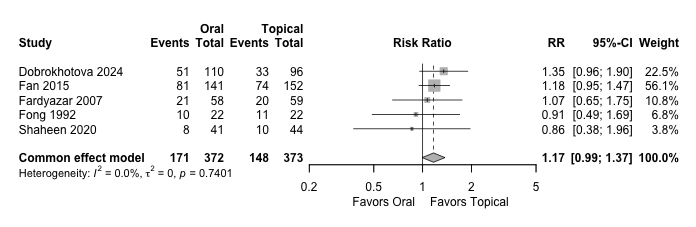
\includegraphics[keepaspectratio]{images/clipboard-3847277273.png}}

}

\caption{\label{fig-forest}Forest plot}

\end{figure}%

Individual study results are shown as boxes centered on their estimate
of effect, with extending horizontal lines indicating their confidence
intervals. The confidence interval expresses the uncertainty around the
point estimate, describing a range of values within which it is
reasonably certain that the true effect lies; wider confidence intervals
reflect greater uncertainty. Although intervals can be reported for any
level of confidence, in most systematic reviews of health interventions,
the 95\% confidence interval is used. Thus, on the forest plot, studies
with wide horizontal lines represent studies with more uncertain
results. Different sized boxes may be plotted for each of the individual
studies, the area of the box representing the weight that the study
takes in the analysis providing a visual representation of the relative
contribution that each study makes to the overall effect.

The plot shows a vertical line of equivalence indicating the value where
there is no difference between groups. For odds ratios, risk ratios or
hazard ratios this line will be drawn at an odds ratio/risk ratio/hazard
ratio value of 1.0, while for risk difference and mean difference it
will be drawn through zero. Studies reach conventional levels of
statistical significance where their confidence intervals do not cross
the vertical line. Summary (meta-analytic) results are presented as
diamonds whose extremities show the confidence interval for the summary
estimate. A summary estimate reaches conventional levels of statistical
significance if these extremities do not cross the line of no effect. If
individual studies are too dissimilar to calculate an overall summary
estimate of effect, a forest plot that omits the summary value and
diamond can be produced.

Odds ratios, risk ratios and hazard ratios can be plotted on a log-scale
to introduce symmetry to the plot. The plot should also incorporate the
extracted numerical data for the groups for each study, e.g.~the number
of events and number of individuals for odds ratios, the mean and
standard deviation for continuous outcomes.

\textbf{Exploring heterogeneity}

There will inevitably be variation in the observed estimates of effect
from the studies included in a meta-analysis. Some of this variation
arises by chance alone, reflecting the fact that no study is so large
that random error can be removed entirely. Statistical heterogeneity
refers to variation other than that which arises by chance. It reflects
methodological or clinical differences between studies. Exploring
statistical heterogeneity in a meta-analysis aims to tease out the
factors contributing to differences, such that sources of heterogeneity
can be accounted for and taken into consideration when interpreting
results and drawing conclusions.

There is inevitably a degree of clinical diversity between the studies
included in a review,160 for example because of differing patient
characteristics and differences in interventions. If these factors
influence the estimated intervention effect, then there will be some
statistical heterogeneity between studies. Methodological differences
that influence the observed intervention effect will also lead to
statistical heterogeneity. For example, combining results from blinded
and un-blinded studies may lead to statistical heterogeneity, indicating
that they might best be analysed separately rather than in combination.
Although it manifests itself in the same way, heterogeneity arising from
clinical differences is likely to be because of differences in the true
intervention effect, whereas heterogeneity arising from differences in
methodology is more likely to be because of bias.

An idea of heterogeneity can be obtained straightforwardly by visually
examining forest plots for variations in effects. If there is poor
overlap between the study confidence intervals, then this generally
indicates statistical heterogeneity.

More formally a X\textsuperscript{2} (chi-squared) test, often also
referred to as Q-statistic, can assess whether differences between
results are compatible with chance alone. However, care must be taken in
interpreting the chi-squared test as it has low power, consequently a
larger P value (P\textless0.1) is sometimes used to designate
statistical significance. Although a statistically significant test
result may point to a problem with heterogeneity, a non-significant test
result does not preclude important between-study differences, and cannot
be taken as evidence of no heterogeneity. Conversely, if there are many
studies in a meta-analysis, the test has high power to detect a small
amount of heterogeneity that, although statistically significant, may
not be clinically important.

Accepting that diversity is likely to be inherent in any review, methods
have also been developed to quantify the degree of inconsistency across
studies, shifting the focus from significance testing to quantifying
heterogeneity.

The I\textsuperscript{2} statistic~is one way to quantify between-study
heterogeneity. The I\textsuperscript{2} statistic is directly based on
Cochran's Q. It is defined as the percentage of variability in the
effect sizes that is not caused by sampling error. Although the
I\textsuperscript{2} statistic often has wide confidence intervals and
it is difficult to provide rules on what level of inconsistency is
reasonable in a meta-analysis, as a rough guide it has been suggested
that I\textsuperscript{2} values of up to 40\% might be unimportant,
30\% to 60\% might be moderate, 50 to 90\% may be substantial and 75\%
to 100\% considerable.

If statistical heterogeneity is observed, then the possible reasons for
differences should be explored and a decision made about if and how it
is appropriate to combine studies. A systematic review does not always
need to include a meta-analysis and, \textbf{\emph{if there are
substantial differences between study estimates of effect, particularly
if they are in opposing directions,}} \textbf{\emph{combining results in
a meta-analysis can be misleading}}.

One way of addressing this is to split studies into less heterogeneous
groups according to particular study level characteristics (e.g.~by type
of drug), and perform separate analyses for each group. Forest plots can
be produced to show subsets of studies on the same plot. Each subset of
studies can have its own summary estimate, and if appropriate an overall
estimate combined across all studies can also be shown. Showing these
groupings alongside each other in this way provides a good visual
summary of how they compare. This approach allows the consistency and
inconsistency between subsets of studies to be examined. Differences can
be summarized narratively, but where possible they should also be
evaluated formally. A X\textsuperscript{2} test for differences across
subgroups can be carried out.

The influence of patient-level characteristics (e.g.~age, gender) or
issues related to equity (e.g.~ethnicity, socioeconomic group) can also
be explored through subgroup analyses, meta-regression or other
modelling approaches. However, there is generally insufficient
information in published study reports to allow full exploration of
heterogeneity in this way and this can usually only be addressed
satisfactorily when IPD are available. Such exploration of heterogeneity
may enable additional questions to be addressed, such as which
particular treatments perform best or which types of patient will
benefit most, but is unlikely to be helpful when there are few studies.
Wherever possible, potential sources of heterogeneity should be
considered when writing the review protocol and possible subgroup
analyses pre-specified rather than trying to explain statistical
heterogeneity after the fact.

\textbf{Subgroup analyses}

Subgroup analyses divide studies (for study level characteristics) or
participant data (for participant level characteristics) into subgroups
and make indirect comparisons between them. These analyses may be
carried out to explore heterogeneity (see above) as well as to try to
answer particular questions about patient or study factors. For example
a subgroup analysis for study level characteristics might examine
whether the results of trials carried out in primary health care
settings are the same as trials carried out in a hospital setting. A
participant level subgroup analysis might examine whether the effect of
the intervention is the same in men as in women.

In individual studies it is unusual to have sufficient numbers and
statistical power to permit reliable subgroup analyses of patient
characteristics. However, provided that such data have been collected
uniformly across studies, a meta-analysis may achieve sufficient power
in each subgroup to permit a more reliable exploration of whether the
effect of an intervention is larger (or smaller) for any particular type
of individual. Although, owing to the multiplicity of testing, these
analyses are still potentially misleading, subgroup analysis within the
context of a large meta-analysis may be the only reasonable way of
performing such exploratory investigations. Not only do the greater
numbers give increased statistical power, but consistency across trials
can be investigated. Indeed, the possibility of undertaking such
analyses is a major attraction of IPD meta-analyses as dividing
participant data into groups for subgroup analysis is seldom possible in
standard reviews of aggregate data. Subgroup analyses in most (non IPD)
systematic reviews focus on grouping according to trial attributes.

The interpretation of the results of subgroup analyses must be treated
with some caution. Even where the original data have come from RCTs, the
investigation of between-study differences is indirect and equivalent to
an observational study. There may be explanations for the observed
differences between groups, other than the attributes chosen to
categorize groupings. Comparisons which are planned in advance on the
basis of a plausible hypothesis and written into the protocol are more
credible than findings that are found through post hoc exploratory
analyses. Furthermore, the likelihood of finding false negative and
false positive significance tests rises rapidly as more subgroup
analyses are done. Subgroups should therefore be restricted to a few
potentially important characteristics where it is reasonable to suspect
that the characteristic will interact with or modify the effect of the
intervention. Note that there is often confusion between prognostic
factors and potential effect modifiers; just because a characteristic is
prognostic does not mean that it will modify the effect of an
intervention. For example, whilst gender is prognostic for survival
(women live longer than men) it does not necessarily mean that women
will benefit more than men will from a drug to treat lung cancer.

\textbf{Meta-regression}

Meta-regression can be used to investigate the effects of differences in
study characteristics on the estimates of the treatment effect, and can
explore continuous as well as categorical characteristics. In principle
it can allow for the simultaneous exploration of several characteristics
and their interactions, though in practice this is seldom possible
because of small numbers of studies. As in any simple regression
analysis, meta- regression aims to predict outcome according to
explanatory variables or covariates of interest. The covariates may be
constant for the entire trial, for example, the protocol dose of a drug,
or a summary measure of attributes describing the patient population,
for example, mean age or percentage of males. The regression is weighted
by precision of study estimates such that larger studies have more
influence than smaller studies.

The regression coefficient is tested to establish whether there is an
association between the intervention effect and the covariate of
interest. Provided that enough data are available (at least 10 studies),
the technique may be a useful exploratory tool.

However, there are limitations. Not all publications will report on all
the covariates of interest (and there could be potential bias associated
with selective presentation of data that have shown a positive
association within a primary study). If a study is missing a covariate
it drops out of the regression, limiting the power and usefulness of the
analysis, which is already likely to be based on relatively few data
points.

Meta-regression is not a good way to explore differences in treatment
effects between different types of individual as summary data may
misrepresent individual participants. What is true of a study with a
median participant age of 60 may not necessarily be true for a
60-year-old patient. Potentially all the benefit could have been shown
in the 50-year-olds and none in the 60 and 70-year-olds. Comparison of
treatment effects between different types of individual, for example
between men and women, should be done using subgroup analyses and not by
using meta-regression incorporating the proportion of women in each
trial. It should always be borne in mind that finding a significant
association in a meta-regression does not prove causality and should
rather be regarded as hypothesis generating.

\textbf{Sensitivity analyses}

Sensitivity analyses explore the robustness of the main meta-analysis
results by repeating the analyses having made some changes to the data
or methods. Analyses run with and without the inclusion of certain
trials will assess the degree to which studies (perhaps those with
poorer methodology) affect the results. For example, analyses might be
carried out on all eligible trials and a sensitivity analysis restricted
to only those that used a placebo in the control group. If results
differ substantially, the final results will require careful
interpretation. However, care must be taken in attributing reasons for
differences, especially when a single or small numbers of trials are
included/excluded in the sensitivity analysis, as a study may differ in
additional ways to the issue being explored in the sensitivity analysis.
Some sensitivity analyses should be proposed in the protocol, but as
many issues suitable for exploration in sensitivity analyses only come
to light whilst the review is being done, and in response to decisions
made or difficulties encountered, these may have to change and/ or be
supplemented.

\textbf{Dealing with special study designs and analysis issues}

\textbf{Intention to treat analyses}

ITT is usually the preferred type of analysis as it is less likely to
introduce bias than alternative approaches. True intention to treat
analysis captures two criteria: (i) participants should be analysed
irrespective of whether or not they received their allocated
intervention and irrespective of what occurred subsequently, for
example, participants with protocol violations or those subsequently
judged ineligible should be included in the analysis; (ii) all
participants should be included irrespective of whether outcomes were
collected. Although the first criterion is generally accepted, there is
no clear consensus on the second as it involves including participants
in the analyses whose outcomes are unknown, and therefore requires
imputation of data. Many authors describe their analyses as ITT when
only the first criterion has been met. Alternative analysis of all
participants for whom outcome data are available is termed available
case analysis. Some studies present analysis of all participants who
completed their allocated treatment, this is per protocol or treatment
received analysis which may be seriously biased.

\textbf{Imputing missing data}

Although statistical techniques are available to impute missing data,
this cannot reliably compensate for missing data and in most situations
imputation of data is not recommended. It is reasonable for most
systematic reviews to aim for an available case analysis and include
data from only those participants whose outcome is known.

Achieving this may require making contact with the study author if
individuals for whom outcome data were recorded have been excluded from
the published analyses. The extent and implications of missing data
should always be reported and discussed in the review. If the number of
participants missing from the final analysis is large it will be helpful
to detail the reasons for their exclusion.

In some circumstances, it might be informative to impute data in
sensitivity analyses to explore the impact of missing data. For missing
dichotomous data the analysis can assume that either all participants
with missing data experienced the event, or that they all did not
experience the event. This generates the theoretical extremes of
possible effect. Data could also be imputed using the rate of events
observed in the control group, however this does not add information,
gives inflated precision and is not recommended. Where missing data are
few, imputation will have little impact on the results. Where missing
data are substantial, analysis of worst/best case scenarios will give a
wide range of possible effect sizes and may not be particularly helpful.

Approaches to imputing missing continuous data have received little
attention. In some cases it may be possible to use last observation
carried forward, or to assume that no change took place. However, this
cannot be done from aggregate data and the value of such analysis is
unclear. Any researcher contemplating imputing missing data should
consult with an experienced statistician.

\textbf{Cluster randomized trials}

In cluster randomized trials, groups rather than individuals are
randomized, for example clinical practices or geographical areas.
Reasons for allocating interventions in this way include evaluating
policy interventions or group effects such as in immunization programs,
and avoiding cross-contamination, for example, health promotion
information may be easily shared by members of the same clinic or
community. In many instances clustering will be obvious, for example
where primary care practices are allocated to receive a particular
intervention. In other situations the clustering may be less obvious,
for example where multiple body parts on the same individual are
allocated treatments or where a pregnant woman has more than one fetus.
It is important that any cluster randomized trials are identified as
such in the review.

As participants within any one cluster are likely to respond in a manner
more similar to each other than to other individuals (owing to shared
environmental exposure or personal interactions), their data cannot be
assumed to be independent. It is therefore inappropriate to ignore the
clustering and analyse as though allocation had been at the individual
level. This unit of analysis error would result in overly narrow
confidence intervals and straightforward inclusion of trials analysed in
this way would give undue weight to that study in a meta-analysis.
Unfortunately, many primary studies have ignored clustering and analysed
results as though from an individual randomized trial. One way to avoid
the problem of inappropriately analysed cluster trials is to carry out
meta-analyses using a summary measure for each cluster as a single
observation. The sample size becomes the number of clusters (not the
number of individuals) and the analysis then proceeds as normal.
However, depending on the size and number of clusters, this will reduce
the statistical power of the analysis considerably and unnecessarily.
Indeed, the information required to do this is unlikely to be available
in many study publications.

A better approach is to adjust the results of inappropriately analysed
primary studies to take account of the clustering, by increasing the
standard error of the estimate of effect. This may be achieved by
multiplying the original standard error by the square root of the
`design effect'. The design effect can be calculated from the
intracluster correlation coefficient, which, although seldom reported,
can use external values from similar studies. A common design effect is
usually adopted across the intervention groups.

These values can then be used in a generic inverse variance
meta-analysis alongside unadjusted values from appropriately analysed
trials.

\textbf{Cross-over trials}

Cross-over trials allocate each individual to a sequence of
interventions, for example one group may be allocated to receive
treatment A followed by treatment B, and the other group allocated to
receive B followed by A. This type of trial has the advantage that each
participant acts as their own control, eliminating between participant
variability such that fewer participants are required to obtain the same
statistical power. They are suitable for evaluating interventions that
have temporary effects in treating stable conditions. They are not
appropriate where an intervention can have a lasting effect that
compromises treatment in subsequent periods of the trial, or where a
condition has rapid evolution, or the primary outcome is irreversible.
The first task of the researcher is to decide whether the cross-over
design is appropriate in assessing the review question.

Appropriate analysis of cross-over trials involves paired analysis, for
example using a paired t-test to analyse a study with two interventions
and two periods (using experimental measurement - control measurement)
for each participant, with standard errors calculated for these paired
measurements. These values can then be combined in a generic inverse
variance meta-analysis. Unfortunately, cross-over trials are frequently
inappropriately analysed and reported.

A common naive analysis of cross-over data is to treat all measurements
on experimental and control interventions as if they were from a
standard parallel group trial. This results in confidence intervals that
are too wide and the trial receives too little weight in the
meta-analysis. However, as this is a conservative approach, it might not
be unreasonable in some circumstances. Where the effect of the first
intervention is thought to have influenced the outcome in subsequent
periods (carry-over), a common approach is to use only the data from the
first period for each individual. However, this will be biased if the
decision to analyse in this way is based on a test of carry-over and
studies analysed in this way may differ from those using paired
analyses. One approach to combining studies with differing types of
reported analyses is to carry out an analysis grouped by type of study
i.e.~grouped by cross-over trial paired analysis, cross-over trial with
first period analysis, parallel group trial, and explore whether their
results differ (see Subgroup analyses above).

Alternatively, the researcher can carry out their own paired analysis
for each trial if

\begin{enumerate}
\def\labelenumi{\arabic{enumi}.}
\item
  the mean and standard deviation or standard error of participant
  differences are available;
\item
  the mean difference plus a t-statistic, p-value or confidence interval
  from a paired analysis is available;
\item
  a graph from which individual matched measurements can be extracted;
  or
\item
  if individual participant data are available.
\end{enumerate}

Another approach is to attempt to approximate a paired analysis by
imputing missing standard errors by `borrowing' from other studies that
have used the same measurement scale or by a correlation coefficient
obtained from other studies or external sources. Researchers will need
to decide whether excluding trials is preferable to inferring data. If
imputation is thought to be reasonable, advice should be sought from an
experienced statistician. Authors should state explicitly where studies
have used a cross-over design and how this has been handled in the
meta-analysis.

\textbf{Mixed treatment comparisons}

Mixed treatment comparisons (MTC), or network meta-analyses, are used to
analyse studies with multiple intervention groups and to synthesize
evidence across a series of studies in which different interventions
were compared. These are used to rank or identify the optimal
intervention. They build a network of evidence that includes both direct
evidence from head-to-head studies and indirect comparisons whereby
interventions that have not been compared directly are linked through
common comparators. A framework has been described that outlines some of
the circumstances in which such syntheses might be considered. Methods
for conducting indirect comparisons and more complex mixed treatment
methods require expert advice. Researchers wishing to undertake such
analyses should consult with an appropriately experienced statistician.

\textbf{Bayesian methods}

Unlike standard analysis techniques, Bayesian analyses allow for the
combination of existing information with new evidence using established
rules of probability. A simple Bayesian analysis model includes three
key elements:

\begin{enumerate}
\def\labelenumi{\arabic{enumi}.}
\item
  Existing knowledge on the effect of an intervention can be retrieved
  from a variety of sources and summarized as a prior distribution
\item
  The data from the studies are used to form the likelihood function
\item
  The prior distribution and the likelihood function are formally
  combined to provide a posterior distribution which represents the
  updated knowledge about the effect of the intervention
\end{enumerate}

Bayesian approaches to meta-analysis may be useful when evidence comes
from a diverse range of sources particularly when few data from RCTs
exist. They can also be used to account for the uncertainty introduced
by estimating the between-study variance in the random-effects model,
which can lead to reliable estimates and predictions of treatment
effects. While there are several good texts available, if a Bayesian
approach is to be used, the advice of a statistical expert is strongly
recommended.

\section{Reporting biases
(Meta-bias)}\label{reporting-biases-meta-bias-1}

Although thorough searches should ensure that a systematic review
captures as many relevant studies as possible, they cannot eliminate the
risk of publication bias. As publication and associated biases can
potentially influence profoundly the findings of a review, the risk of
such bias should be considered in the review's conclusions and
inferences.

The obvious way to test for publication bias is to compare formally the
results of published and unpublished studies. However, more often than
not unpublished studies are hidden from the reviewer, and more ad hoc
methods are required. A common technique to help assess potential
publication bias is the funnel plot.

This is a scatter plot based on the fact that precision in estimating
effect increases with increasing sample size. Effect size is plotted
against some measure of study precision - of which standard error is
likely to be the best choice. A wide scatter in results of small
studies, with the spread narrowing as the trial size increases, is
expected. If there is no difference between the results of small and
large studies, the shape of the plot should resemble an inverted funnel
(Figure~\ref{fig-funnel-sym}). If there are differences, the plot will
be skewed and a gap where the small unfavorable studies ought to be is
often cited as evidence of publication bias
(Figure~\ref{fig-funnel-asym}). However, the shape of a funnel plot can
also depend on the measures selected for estimating effect and precision
and could be attributable to differences between small and large studies
other than publication bias. These differences could be a result of
other types of methodological bias (Figure~\ref{fig-funnel-small}), or
genuine clinical differences. For example, small studies may have a more
selected participant population where a larger treatment effect might be
expected. Funnel plots are therefore more accurately described as a tool
for investigating small study effects.

\begin{figure}

\centering{

\pandocbounded{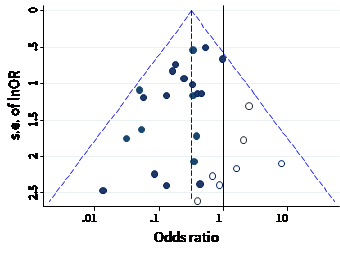
\includegraphics[keepaspectratio]{images/clipboard-4161934926.png}}

}

\caption{\label{fig-funnel-sym}Symmetrical plot in the absence of bias
due to missing evidence}

\end{figure}%

\begin{figure}

\centering{

\pandocbounded{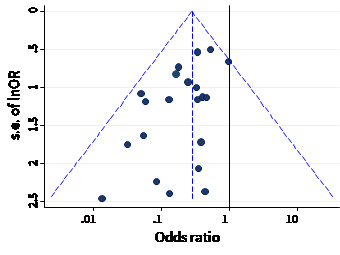
\includegraphics[keepaspectratio]{images/clipboard-1538892079.png}}

}

\caption{\label{fig-funnel-asym}Asymmetrical plot in the presence of
bias due to missing evidence}

\end{figure}%

\begin{figure}

\centering{

\pandocbounded{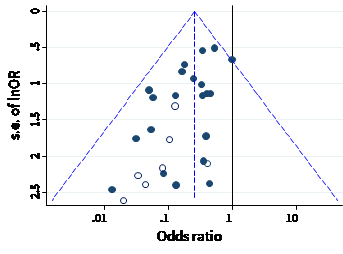
\includegraphics[keepaspectratio]{images/clipboard-2657010065.png}}

}

\caption{\label{fig-funnel-small}Asymmetrical plot in the presence of
bias because some smaller studies (open circles) had flaws and therefore
produced exaggerated intervention effect estimates}

\end{figure}%

Although visual inspection of funnel plots has been shown to be
unreliable, this might be improved if contour zones illustrating
conventional levels of significance are overlaid on the plot to
illustrate whether `missing' studies are from zones of statistical
significance or not. If the `missing' studies are from non-significant
zones, this may support a publication bias. On the other hand if
`missing' studies are from statistically significant zones, the
asymmetry may be more likely to be attributable to other causes.

A range of statistical and modelling methods have been developed to test
for asymmetry, the most frequently used of which are those based on rank
correlation or linear regression and complex modelling methods.

Some methods (for example, the trim and fill method) attempt to adjust
for any publication bias detected. However, all methods are by nature
indirect and the appropriateness of many methods is based on some strict
assumptions that can be difficult to justify in practice.

Although frequently used to help assess possible publication bias,
funnel plots and associated statistical tests are often used and
interpreted inappropriately, potentially giving false assurance where a
symmetrical plot overlooks important bias or undermining important valid
evidence because of an asymmetric plot. The methods are inappropriate
where there is statistical heterogeneity; have low power and are of
little use where there are few studies; and are meaningless where
studies are of similar size. Consequently, situations where they are
helpful are few and their use is not generally a good way of dealing
with publication bias. Therefore use of these methods to identify or
adjust for publication bias in a meta-analysis should be considered
carefully and generally be restricted to sensitivity analyses. Results
should be interpreted with caution. Statistical tests will not resolve
bias and avoidance of publication bias is preferable. In time this may
become easier with more widespread registration of clinical trials and
other studies at inception.

\section{Certainty of evidence}\label{certainty-of-evidence-1}

The authors should use the Grading of Recommendations, Assessment,
Development and Evaluation (GRADE) approach to create the Summary of
Findings. GRADE uses study limitations, consistency of effect,
imprecision, indirectness, and publication bias to assess the certainty
of evidence for each outcome. A summary of the intervention effect and a
measure of certainty should be produced using the GRADE Profiler
Guideline Development Tool (GRADEpro GDT) software for the prespecified
important outcomes. (GRADEpro 2025)

\section{Interpreting results}\label{interpreting-results}

When describing review findings, the results of all analyses should be
considered as a whole, and overall coherence discussed. Consistency
across studies should be considered and results interpreted in relation
to biological and clinical plausibility.

Where there have been many analyses and tests, care should be taken in
interpreting unexpected or implausible findings as among a large number
of tests the play of chance alone is likely to generate spurious
statistically significant results.

Quantitative results of meta-analyses should be expressed as point
estimates together with associated confidence intervals and exact
p-values. They should not be presented or discussed only in terms of
statistical significance. This is particularly important where results
are not statistically significant as nonsignificance can arise both when
estimates are close to no effect with narrow confidence intervals, or
when estimates of effect are large with wide confidence intervals.
Whilst in the former, we can be confident that there is little
difference between the interventions compared, in the latter there is
insufficient evidence to draw conclusions. Researchers should be aware
that describing a result as `there is no statistical (or statistically
significant) difference between the two interventions' can be (mis)read
as there being no difference between interventions.

It is important that inconclusive results are not interpreted as
indicating that an intervention is ineffective and estimates with wide
confidence intervals that span no effect should be described as showing
no clear evidence of a benefit or harm rather than as there being no
difference between interventions. Demonstrating lack of sufficient
evidence to reach a clear conclusion is an important finding in its own
right.

Similarly, care should be taken not to overplay results that are
statistically significant, as with large enough numbers, even very
modest differences between interventions can be statistically
significant. The size of the estimated effect, and its confidence
intervals, should be considered in view of how this relates to current
or future practice.

It is usually helpful to present findings in both relative and absolute
terms and in particular to consider how relative effects may translate
into different absolute effects for people with differing underlying
prognoses (see Relative and absolute effects section above). Where a
number of outcomes or subgroup analyses are included in a review it can
be helpful to tabulate the main findings in terms of effect, confidence
intervals and inconsistency or heterogeneity statistics.

\textbf{Summary: Data synthesis}

\begin{itemize}
\item
  Synthesis involves bringing the results of individual studies together
  and summarizing their findings.
\item
  This may be done quantitatively or, if formal pooling of results is
  inappropriate, through a narrative approach.
\item
  Synthesis should also explore whether observed intervention effects
  are consistent across studies, and investigate possible reasons for
  any inconsistencies.
\item
  Initial descriptive synthesis

  \begin{itemize}
  \tightlist
  \item
    All syntheses should begin by constructing a clear descriptive
    summary of the included studies.
  \end{itemize}
\item
  Narrative synthesis is an essential part of a systematic review, and
  as with every other stage of the process, bias must be minimized.

  \begin{itemize}
  \item
    A general framework can be applied in order to help maintain
    transparency and add credibility to the process. The four elements
    of this framework are:

    \begin{itemize}
    \item
      Developing a theory of how the intervention works, why and for
      whom
    \item
      Developing a preliminary synthesis of findings of included studies
    \item
      Exploring relationships within and between studies
    \item
      Assessing the robustness of the synthesis
    \end{itemize}
  \item
    Each element contains a range of tools and techniques that can be
    applied. A researcher is likely to move iteratively among the four
    elements, choosing those tools and techniques that are appropriate
    to the data being synthesized and providing justifications for these
    choices.
  \end{itemize}
\item
  Quantitative synthesis

  \begin{itemize}
  \item
    Meta-analysis increases power and precision in estimating
    intervention effects.
  \item
    Results of individual studies are combined statistically to give a
    pooled estimate of the `average' intervention effect.
  \item
    Most meta-analysis methods are based on calculating a
    \textbf{\emph{weighted average}} of the effect estimates from each
    study.
  \item
    The methods used to combine results will depend on the type of
    outcome assessed.
  \item
    Quantitative results should be expressed as point estimates together
    with associated confidence intervals and exact p-values.
  \item
    Variation in results across studies should be investigated.
  \item
    Sensitivity analyses give an indication of the robustness of results
    to the type of study included and the methods used.
  \end{itemize}
\end{itemize}

\section{Report writing}\label{report-writing}

Report writing is an integral part of the systematic review process. The
report should describe the review methods clearly and in sufficient
detail that others could, if they wished, repeat them. There is evidence
that the quality of reporting in reports of primary studies may affect
the readers' interpretation of the results, and the same is likely to be
true of systematic reviews. It has also been argued that trials and
reviews often provide incomplete or omit the crucial `how to' details
about interventions, limiting a clinicians' ability to implement
findings in practice. PRISMA (Preferred Reporting Items for Systematic
Reviews and Meta- Analyses), flow chart, and checklist, provide guidance
for the reporting of systematic reviews with or without a meta-analysis.
(Page et al. 2021)

\textbf{Style and structure}

Commissioning bodies and journals usually have specific requirements
regarding presentation and layout that should be followed when preparing
a report or article. Some organisations offer detailed guidance while
others are less specific. In the absence of guidance, a layered approach
such as a one page summary of the research `actionable messages',
three-page executive summary and a 25-page report is advocated as the
optimal way to present research evidence to health service managers and
policy-makers.

Many journals publish papers electronically ahead of print publication
and electronic publishing often allows additional material, such as
large tables, or search strategies to be made available through the
journal's website. There is no specific word limit for reports published
in electronic format only, for example in the Cochrane Library, although
Cochrane reviews `should be as succinct as possible'.

Researchers should familiarize themselves with the conventions favored
by their commissioning body or `target' journal. Many journals now
prefer a clear and active style that is understandable to a general
audience. Weaknesses in the use of grammar and spelling constitute
obstacles to clear communication and should be eliminated as far as
possible. The field of scientific and technical communication
predominantly uses English as its common language, so those who are
unsure of their ability in written English may find it helpful to have
their report checked by an accomplished speaker/ writer who is familiar
with the subject matter before submission.

Contents lists and headings are essential for guiding the reader through
longer documents. Inclusion of an index may also be helpful. It is
particularly important to adopt a consistent style (e.g.~font, point
size, font style) for different levels of main headings and
sub-headings.

\textbf{Planning}

Time spent preparing a brief outline covering the main points to be
included in the report can save time overall. The outline should focus
on who the intended audience is and what they need to know. The review
team will need to agree the outline and, if the report is to be written
by multiple authors, allocate writers for each section. Dividing the
work amongst a number of people reduces the burden on each individual
but there is a risk of loss of consistency in style and terminology. In
addition, completion of the report relies on all the team members
working to the agreed schedule. It is essential for the lead author
(corresponding author for journal articles) to monitor progress and take
responsibility for accuracy and consistency.

\textbf{Authors and contributors}

The report of a systematic review will usually have a number of authors.
The ICMJE (ICMJE 2025) recommends that authorship be based on the
following 4 criteria:

\begin{itemize}
\item
  Substantial contributions to the conception or design of the work; or
  the acquisition, analysis, or interpretation of data for the work; AND
\item
  Drafting the work or reviewing it critically for important
  intellectual content; AND
\item
  Final approval of the version to be published; AND
\item
  Agreement to be accountable for all aspects of the work in ensuring
  that questions related to the accuracy or integrity of any part of the
  work are appropriately investigated and resolved.
\end{itemize}

In addition to being accountable for the parts of the work done, an
author should be able to identify which co-authors are responsible for
specific other parts of the work. In addition, authors should have
confidence in the integrity of the contributions of their co-authors.

All authors should meet all of these conditions. The review team should
agree among themselves who will be authors and the order of authorship.
Order of authorship is often taken to reflect an individual's
contribution to the report and methods are available for scoring
contributions to determine authorship. Alternatively authors can simply
be listed alphabetically. Contributions that do not meet the criteria
for authorship (e.g.~data extraction or membership of an advisory group)
should be included in the acknowledgements.

\textbf{Conflict of interests}

The ICMJE state that a conflict of interests exists if `an author (or
the author's institution), reviewer, or editor has financial or personal
relationships that inappropriately influence (bias) his or her actions'.
Relationships that might constitute a conflict of interests are common
and there is nothing wrong with having such relationships. However, it
is important that they are declared so that readers are aware of the
possibility that authors' judgments may have been influenced by other
factors. Review authors need to be explicit about any potential conflict
of interests because such transparency is important in maintaining the
readers' confidence. (ICMJE 2025)

\textbf{Executive summary or abstract}

The executive summary (for full-length reports) or abstract (for journal
articles) is the most important part of the report because potentially
it is the only section that many readers will actually read (perhaps in
conjunction with the discussion and conclusions). It should present the
findings of the review clearly and concisely and allow readers to
quickly judge the quality of the review and the generalizability of its
findings. Providing a good balance between detail of the intervention
and how the review was conducted, and the results and conclusions is
always a challenge, and may require several iterations across the whole
review team. The summary is usually the last section to be written so
that full consideration can be given to all relevant aspects of the
project. However, the process of summary writing may help in the further
development of the recommendations by forcing review teams to identify
the one or two most important findings and the conclusions which flow
from them. It should be remembered that revisions to the report or
article following peer review may also need to be reflected in the
summary. Assistance from outside parties and medical writers may be
helpful in developing a good summary.

\textbf{Formulating the discussion}

The purpose of the discussion section of a report is to help readers to
interpret the results of the review. This should be done by presenting
an analysis of the findings and outlining the strengths and weaknesses
of the review. The discussion should also place the findings in the
context of the existing evidence base, particularly in relation to any
existing relevant reviews. It has been suggested that more could and
should be done in discussion sections to contextualize both the nature
of the research and the findings to the existing evidence base. There
should be a balance between objectively describing the results, and
subjectively speculating on their meaning. It is important to present a
clear and logical train of thought and reasoning, supported by the
findings of the review and other existing knowledge.

\textbf{Conclusions, implications, recommendations}

Faced with the need to make decisions and limited time to read the whole
report, many readers may go directly to the conclusions. Therefore,
whether incorporated in the discussion section or presented separately,
it is essential that the conclusions be clearly worded and based solely
on the evidence reviewed.

The conclusions should summarize the evidence and draw out the
implications for health care, and preferably be worded to show how they
have been derived from the evidence.

We advise authors to follow the model of Cochrane reviews when drafing
the conclusions. Authors' conclusions from Cochrane reviews are
presented as the implications for practice and research; recommendations
are not made. Recommendations for practice are usually only made in
guidelines, and are formulated from a variety of sources of information
in addition to review findings.

A clear statement of the implications for future research should be
made; vague statements along the lines of `more research is needed' are
not helpful and should be avoided. Specific gaps in the evidence should
be highlighted to identify the research questions that need answering.
Where methodological issues have been identified in existing studies,
suggestions for future approaches may be made. Where possible, research
recommendations should be listed in order of priority, and an indication
of how rapidly the knowledge base in the area is developing should be
included. This can assist in planning an update of the review and help
guide commissioners when allocating funding.

\textbf{Summary: Report writing}

\begin{itemize}
\item
  Report writing is an integral part of the systematic review process.
\item
  Reviews may be published as a report for the commissioner, as a
  journal article or both.
\item
  Readability is a key aspect of reporting; a review's findings will not
  be acted on if they are not clearly presented and understood.
\item
  The executive summary (for full-length reports) or abstract (for
  journal articles) is the most important part of the report, because it
  is potentially the only section that many readers will actually read
  (perhaps in conjunction with the discussion and conclusions).
\item
  Implications for practice or policy and recommendations for further
  research should be based solely on the evidence contained in the
  review.
\item
  The findings from systematic reviews are frequently used to inform
  guideline development. Guideline recommendations are often formulated
  using a grading scheme. Systematic review reports should therefore aim
  to provide the information required for such grading schemes.
\end{itemize}

\part{Reviews of Clinical Tests}

\chapter{Reviews of clinical tests}\label{reviews-of-clinical-tests-1}

Healthcare professionals use clinical tests for diagnosis, confirming or
excluding the presence of a disease or condition. They also use clinical
tests to monitor disease progression, assess prognosis, and screen
asymptomatic populations for disease. Any process that yields
information used to inform patient management can be regarded as a
clinical test. This includes a wide range of processes from history
taking and physical examination to complex imaging techniques. The test
forms part of the continuum of patient care.

New tests are adopted into clinical practice for a number of reasons,
including \textbf{replacement} of an existing test (where the new test
is expected to reduce the negative impact on the patient, provide better
information, or equivalent information for less cost), \textbf{triage}
(to decide whether a more expensive or invasive test is necessary), or
as an \textbf{add-on} (addition to the existing testing protocol to
increase the accuracy of a testing strategy).

The ultimate aim of any research on clinical tests should be to
determine impact upon patient management and outcome. To date much of
the research on clinical tests is in the form of test accuracy studies.
The basic aim of test accuracy studies is to assess how well a test can
distinguish between people with and without the disease/condition of
interest. The outcome measures used describe the probabilistic
relationships between positive and negative test results, and the
presence or absence of disease, as compared with the best currently
available method (i.e.~the reference test).

When considering a systematic review of test accuracy studies, it is
important to assess whether review findings will be able to provide the
information necessary to inform clinical practice. Any review of test
accuracy is likely to be of limited value where evidence is lacking that
the disease/condition is associated with long-term morbidity or
mortality, or where no effective intervention is available.

\section{The review question}\label{the-review-question}

As with all systematic reviews, the development of a clear, well-defined
question is essential to maintaining transparency of the review process
and to the quality and relevance of the findings.

We prefer the alternative acronym PIT for test accuracy questions, where
the three letters refer to population, index test(s) and target
condition. P describes the persons for whom the test is considered, and
may include the healthcare setting and tests done prior to using the
index test. We prefer `population' rather than `patients', because tests
may also be used in asymptomatic persons, as in population screening
programmes. I describes the index test(s). T describes the target
condition. These three elements are further explained below.

\subsection{From question to
objectives}\label{from-question-to-objectives}

The primary objective will typically refer to the accuracy of the index
test(s) for the diagnosis of the target condition in the relevant
population.

\textbf{Example}:

\textbf{\emph{Review question}}: In immuno-compromised patients (P), is
measuring galactomannan in blood (I) sufficiently sensitive to serve as
a triage test for fungal disease (T)?

\textbf{\emph{Objective}}: To assess the diagnostic accuracy of
galactomannan detection in serum for the diagnosis of invasive
aspergillosis in immuno-compromised patients, at different cut‐off
values for test positivity.

\section{Eligibility criteria}\label{eligibility-criteria-1}

\textbf{Population}

Clinical tests perform differently in different populations, for example
it would generally be inappropriate to evaluate the performance of a
test in a secondary care population when the test is mainly used in
primary care. Both frequency and severity of the target condition would
be expected to be greater in secondary care. It is therefore important
to clearly define the population of interest.

The ideal study sample for a test accuracy study is a consecutive or
randomly selected series of patients in whom the target condition is
suspected, or for screening studies, the target population.

Because participant sampling methods are often poorly reported in test
accuracy studies, using the sampling method as an inclusion/exclusion
criterion in the review is likely to result in a substantial reduction
in available data. It is likely to be more useful to consider the
sampling method and/or its reporting as an aspect of study quality and
to base the inclusion criteria relating to the population upon
participant characteristics. For example in a review comparing the
accuracy of different imaging techniques, the inclusion criteria might
state that only patients with a specified level of symptoms,
representative of those in whom the test would be used for intervention
planning, are eligible.

\textbf{Index test}

As with any review, the scope of the question can be broad such as `what
is the optimum testing pathway for the diagnosis and follow-up
investigation of childhood urinary tract infection (UTI)?' or it can be
narrow; for example `what is the diagnostic accuracy of magnetic
resonance angiography (MRA) when compared with intra-arterial x-ray
angiography, for the detection of carotid artery stenosis?' The former
is likely to include a number of different technologies, addressing
multiple target conditions, whereas the latter compares the performance
of an alternative (replacement), less invasive or less costly diagnostic
technology with that of the reference standard for the detection of a
specified target condition. The rate of technological development may be
an important consideration; in this latter example inclusion of MRA
techniques that are already obsolete in clinical practice, is unlikely
to be useful.

Careful consideration should always be given to the equivalence of
different analytical techniques when setting inclusion criteria. For
example, a systematic review of fecal occult blood tests to screen for
colorectal cancer evaluated both immunochemical and colourimetric
methods for detecting blood in the feces; though both methods target
blood, they cannot be considered equivalent tests.

The traditional concept of test accuracy often implies the
dichotomization of data into test results which are classified as
positive (target condition present) or negative (target condition
absent). Any systematic review of test accuracy will therefore need to
consider diagnostic thresholds (points at which results are classified
as positive or negative) for each included index test.

\textbf{Reference standard}

The reference standard is usually the best test currently available, and
is the standard against which the index test is compared. It needs not
be the test used routinely in practice (although it can be).

The test accuracy study is based upon a one-sided comparison between the
results of the index test and those of the reference standard. Any
discrepancy is assumed to arise from error in the index test. Selection
of the reference standard is therefore critical to the validity of a
test accuracy study and the definition of the diagnostic threshold forms
part of that reference standard.

Note that the assumption of 100\% accuracy for the reference standard
rarely holds true in practice. This represents a fundamental flaw in the
test accuracy study design, since the index test can never be deemed to
perform better than the reference standard, and its value may therefore
be underestimated.

Where several tests are available to diagnose the target condition,
there is often no consensus about which test constitutes the reference
standard. In such cases a composite reference standard, which combines
the results of several available tests to produce a better indicator of
true disease status may be used.

In some instances, it is deemed unethical to use an invasive procedure
as a reference standard in a study. In such cases, clinical follow-up
and final diagnosis may sometimes be used as a reference standard. There
will also be occasions when clinical follow-up and final diagnosis
provides the most appropriate reference standard. The length of
follow-up should ideally be defined in advance. Studies using follow-up
and clinical outcome in this way may be viewed as prognostic studies in
that they are measuring the accuracy with which the test is able to
predict a future event, rather than the accuracy with which it is able
to determine current status. Where such studies are included in a
systematic review, it is important to define, in advance, what
constitutes appropriate follow-up and hence an adequate reference
standard.

The index test may also be evaluated against the test currently in
practice. Ideally, this should be done by comparing index test and
currently available test to the reference standard in the same
population.

\textbf{Outcome measures}

The primary outcome of interest for any systematic review of test
accuracy is the data required to populate 2 x 2 contingency tables.
These describe the relationship between the results of the index test
and the reference standard at a given diagnostic threshold (point at
which results are classified as positive or negative). The table
includes the number of true positives (TP: those that have the disease
and test positive), false positives (FP: those that do not have the
disease and test positive), false negatives (FN: those that do have the
disease and test negative) and true negatives (TN: those that do not
have the disease and test negative).

\begin{longtable}[]{@{}llll@{}}
\toprule\noalign{}
\endhead
\bottomrule\noalign{}
\endlastfoot
& & Reference standard & \\
& & Disease & No disease \\
Index test & Positive & TP & FP \\
& Negative & FN & TN \\
\end{longtable}

From the 2 x 2 contingency table (AKA confusion matrix), the following
commonly used measures of test performance can be calculated:
sensitivity (true positive proportion, A test with a higher sensitivity
has a lower type II error rate), specificity (true negative proportion,
a test with a higher specificity has a lower type I error rate),
diagnostic accuracy (the correctly classified proportion), diagnostic
odds ratio, the number needed to diagnose, positive predictive value
(precision), negative predictive value, Likelihood ratio of a positive
test (LR+), and Likelihood ratio of a negative test (LR-).

In primary studies, a receiver operating characteristic (ROC) curve
describes the relationship between `true positive fraction'
(sensitivity) and `false positive fraction' (1- specificity) for
different positivity thresholds. It is used to display the trade-offs
between sensitivity and specificity as a result of varying the
diagnostic threshold.

In some scenarios (e.g.~tests used in population screening) a threshold
which skews diagnostic performance may be preferable (e.g.~minimizing
the number of false negatives at the expense of some increase in the
number of false positive results, in conditions/diseases where missing
the presence of disease will lead to serious consequences). Overall
diagnostic accuracy is summarized by the area under the curve (AUC); the
closer the curve is to the upper left hand corner the better the
diagnostic performance. The AUC ranges from 0 to 1, with 0.5 indicating
a poor test where the accuracy is equivalent to chance.

As with other types of intervention, when assessing the clinical
effectiveness of a diagnostic test, it is important to consider all
outcome measures which may be relevant to the use of the test in
practice. These might include adverse events and the preferences of
patients, although inclusion of such information is rare.

\textbf{Study design}

There are two basic types of test accuracy study: `single-gate' which
are similar to consecutive series and `two-gate' which are similar to
case-control studies. The term `two-gate' being used where two sets of
inclusion criteria or `gates' are applied, one for participants who have
the target condition and one for those who do not. These designs differ
in structure from other cohort and case-control studies in that both are
generally cross-sectional in nature.

\begin{itemize}
\item
  The single-gate design includes participants in whom \textbf{\emph{the
  disease status is unknown}}, and compares the results of the index
  test with those of the reference standard used to confirm diagnosis,
  i.e.~it is broadly representative of the scenario in which the test
  would be used in practice.
\item
  The two-gate design compares the results of the index test in patients
  with an established diagnosis of the target condition with its results
  in healthy controls or controls with another diagnosis (known status,
  with respect to the target condition, is therefore treated as the
  reference standard); i.e.~it is unrepresentative of practice and is
  unlikely to contain the full spectrum of health and disease over which
  the test would be used.
\end{itemize}

There are inherent problems with the two-gate design that may lead to
bias. The selective inclusion of cases with more advanced disease is
likely to lead to over estimations of sensitivity and inclusion of
healthy controls is likely to lead to over estimations of specificity.
The recruitment of healthy controls from the general population has been
associated with two- to three-fold increases in measures of test
performance time-to-events derived from a diagnostic cohort design. This
over estimation can be increased further when cases of severe disease
are used alongside healthy controls. By contrast, where cases are
derived from individuals with mild disease, underestimations of
sensitivity can result. Where the control group is derived from patients
with alternative diagnoses, specificity may be under or overestimated,
depending upon the alternative diagnosis. In theory, the two-gate study
design could produce a valid estimate of test performance if the cases
were sampled to match the reference standard positive patients in a
single-gate study (in terms of the spectrum of disease severity) and
controls were matched to the reference standard negative patients (in
terms of the spectrum of alternative conditions). In practice however,
this is difficult to achieve. Whilst two-gate studies are therefore of
limited use in assessing how a test is likely to perform in clinical
practice, they can be useful in the earlier phases of test development.
Where systematic reviews include both single and two-gate study designs,
careful consideration should be given to the methods of analysis and the
impact of study design should be assessed in any meta-analyses.

\section{Identifying research
evidence}\label{identifying-research-evidence-1}

\textbf{Sources}

The importance of searching a wide range of databases to avoid missing
relevant diagnostic test accuracy studies has been demonstrated, with
MEDLINE and EMBASE providing unique records. The reference lists of
included studies can also be a useful resource.

\textbf{Database searching}

Many electronic databases do not have appropriate indexing terms to
label test accuracy studies, and those that do tend not to apply them
consistently. They also vary in their design which adds to the
difficulty in identification. The problem is compounded by the fact that
the original authors might inadequately reporting and labeling their
studies as being test accuracy.

The use of filters to identify reports of diagnostic test accuracy
studies in electronic databases may miss a considerable number of
relevant articles and is therefore not generally considered appropriate.
Database searching should concentrate on terms for index tests and
target conditions. If further restriction is required, it can be
achieved by means of topic specific terms, rather than using a filter.
It is hoped, however, that in time, as the issues of reporting and
indexing diagnostic, screening, and prognostic studies are more widely
realized, the situation will improve allowing the development of more
accurate filters.

\textbf{Publication bias}

As the data used in studies of test accuracy are often collected as part
of routine clinical practice (and in the past have tended not to require
formal registration) it has been argued that test accuracy studies are
more easily conducted and abandoned than RCTs. They may therefore be
particularly susceptible to publication bias.

It has been demonstrated that the unique features of the test accuracy
study make the application of the Begg, Egger, and Macaskill tests of
funnel plot asymmetry potentially misleading. An alternative approach
uses funnel plots of (natural logarithm (ln) DOR) vs.~(1/√effective
sample size) and tests for asymmetry using related regression or rank
correlation tests. It should be noted that the power of all statistical
tests for funnel plot asymmetry decreases with increasing heterogeneity
of DOR. It should also be noted that factors other than publication
bias, for example aspects of study quality and population
characteristics, may be associated with sample size.

Given the limitations of current knowledge, to ignore the possibility of
publication bias would seem unwise, however, its assessment in reviews
of test accuracy is complex.

\section{Data extraction}\label{data-extraction-1}

The same precautions against reviewer bias and error should be employed
whilst extracting data from test accuracy studies as would be applied in
any other type of review. Independent checking of 2x2 data is
particularly important, as test accuracy studies are often poorly
reported, and the production of a 2x2 table from these studies can be
challenging.

Some studies may provide the actual results for each test for individual
patients. In this case the researcher may need to classify each patient
according to the diagnostic thresholds defined in the review protocol.

Studies may provide categorical data, which may represent multiple
categories or stages of disease. In this case data will need to be
extracted for the numbers of index test positive and negative
participants (using the threshold(s) defined in the review protocol,
which may include all thresholds reported) with and without the target
condition (as defined by the reference standard, using the threshold(s)
defined in the review protocol).

There may be instances when the raw data are not reported, but 2x2 data
can be calculated from reported accuracy measures and total numbers of
diseased or non- diseased patients.

Somewhat more problematic are cases when the data do not `fit' the 2x2
contingency table model. `Forcing' data into a 2x2 contingency table,
for example by classifying uncertain index test results as FP or FN, may
be inappropriate. The contingency table can be extended to form a six
cell table, which accommodates uncertain or indeterminate index test
results.

The informative value of an indeterminate test result can be assessed
using an indeterminate likelihood ratio (or LR+/-), defined as the
probability of an indeterminate test result in the presence of disease
divided by the probability of an indeterminate test result in the
absence of disease.

When index test and reference standard give clear results (i.e.,
considered determinate), but there is incomplete concordance, the 2x2
table may be expanded to accommodate a more complete clinical picture.

\section{Methodological quality}\label{methodological-quality}

Structured appraisal of methodological quality is key to assessing the
reliability of test accuracy studies included in a systematic review.
Quality assessment should consider the association of individual
elements of methodological quality with test accuracy; generating
overall `quality scores' is not recommended.

There are many differences in the design and conduct of diagnostic
accuracy studies that can affect the interpretation of their results.
Some differences lead to systematic bias such that estimates of
diagnostic performance will differ from their true values, others give
rise to variation in results between studies, which can limit
applicability. The distinction between bias and variation is not always
clear, and the risk of assessment checklists have tended to include
items that are pertinent to both. Whilst it is clear that variation
(e.g.~in the demographic characteristics or severity of disease in the
study population) can affect the applicability of the results of both
individual studies and systematic reviews, there is limited evidence on
the effects of design-related biases in primary studies on the results
of systematic reviews. Research on the impact of design-related biases
is largely a work in progress, being dependent upon the availability of
adequate data sets and consistent methods of quality assessment.

\subsection{Sources of bias and variation in test accuracy
studies}\label{sources-of-bias-and-variation-in-test-accuracy-studies}

Variation

\begin{itemize}
\item
  Population

  \begin{itemize}
  \item
    Demographic characteristics: Test may perform differently in
    different populations.
  \item
    Disease severity: Differences in disease severity may lead to
    different estimates of diagnostic performance.
  \item
    Participant selection: A selection process that may not include a
    spectrum of patients similar to that in which the test will be used
    in practice may limit the applicability of study findings.
  \end{itemize}
\item
  Analysis

  \begin{itemize}
  \tightlist
  \item
    Arbitrary choice of threshold value: The diagnostic threshold is
    derived from the same data set in which test performance is
    evaluated. The choice of a threshold value based upon that which
    maximizes sensitivity and specificity for the study data may result
    in exaggerated estimates of test performance. The test may perform
    less well at the chosen threshold when evaluated in a new
    independent patient set.
  \end{itemize}
\item
  Application of the reference standard

  \begin{itemize}
  \tightlist
  \item
    Observer: The interpretation placed upon a test result may vary
    between observers and this can affect estimates of test accuracy.
    The reproducibility of a test within (intra) and between (inter)
    observers affects its applicability in practice.
  \end{itemize}
\item
  Test methods

  \begin{itemize}
  \item
    Technological: Diagnostic performance of tests can change over time
    due to technological improvements.
  \item
    Test execution: Differences in the execution of the index test
    and/or reference standard can result in different estimates of
    diagnostic performance; clear reporting of the methods used is
    therefore important.
  \end{itemize}
\end{itemize}

Bias

\begin{itemize}
\item
  \textbf{Population}

  \begin{itemize}
  \tightlist
  \item
    Disease prevalence: The prevalence of the target condition varies
    with the setting and may affect estimates of diagnostic performance.
    In settings of higher prevalence, interpreters are more prone to
    classify test results as abnormal (context bias).
  \end{itemize}
\item
  \textbf{Analysis}

  \begin{itemize}
  \tightlist
  \item
    Handling of un-interpretable results: Diagnostic tests fail or
    produce un-interpretable results with varying frequency. Study
    participants for whom a test result could not be obtained are often
    removed from reported analyses. This may lead to a biased assessment
    of test performance.
  \end{itemize}
\item
  \textbf{Application of the reference standard}

  \begin{itemize}
  \item
    Clinical review: The availability of other relevant clinical
    information (e.g.~symptoms, co-morbidities) may also affect
    estimates of test performance.
  \item
    Differential verification: Occurs when the diagnosis is verified
    using different reference standards, depending upon the result of
    the index test.
  \item
    Incorporation: Occurs when the result of the index test is used in
    establishing the final diagnosis (i.e.~it forms part of the
    reference standard).
  \item
    Partial verification: Occurs where only a selected sample of
    participants undergoing the index test also receive the reference
    standard.
  \item
    Test or diagnostic review: Where interpretation of either the index
    test or reference standard may be influenced by knowledge of the
    results of the other test. Diagnostic review bias may be present
    when the results of the index test are known to those interpreting
    the reference standard. Test review bias may be present when the
    results of the reference standard are known to those interpreting
    the index test.
  \item
    Use of an inappropriate reference standard: The error in diagnoses
    derived from an imperfect reference standard can result in
    underestimation of the performance of the index test.
  \end{itemize}
\item
  \textbf{Test methods}

  \begin{itemize}
  \item
    Disease progression: Occurs when there is sufficient time delay
    between the application of the index test and the reference standard
    to allow change in the disease state.
  \item
    Treatment paradox: Occurs when treatment is started, based upon the
    results of one test prior to undertaking the other; thus disease
    state is potentially altered between tests.
  \end{itemize}
\end{itemize}

\subsection{Risk of bias assessment}\label{risk-of-bias-assessment-2}

QUADAS is an evidence-based, validated, quality assessment tool
specifically for use in systematic reviews of test accuracy studies. The
QUADAS-2 (Whiting et al. 2011) criteria and the sources of bias and
variation to which they relate are shown in Table~\ref{tbl-quad}.
Piloting of the quality assessment process on a small sample of included
studies should be done in an attempt to eliminate any discrepancies in
understanding between reviewers.

QUADAS-2 has four domains.

\begin{enumerate}
\def\labelenumi{\arabic{enumi}.}
\item
  \textbf{Patient Selection:}

  \begin{itemize}
  \item
    Describe methods of patient selection.
  \item
    Describe included patients (previous testing. presentation, intended
    use of index test, and setting)
  \end{itemize}
\item
  \textbf{Index Test}

  \begin{itemize}
  \tightlist
  \item
    Describe the index test and how it was conducted and interpreted
  \end{itemize}
\item
  \textbf{Reference Standard}

  \begin{itemize}
  \tightlist
  \item
    Describe the reference standard and how it was conducted and
    interpreted
  \end{itemize}
\item
  \textbf{Flow and Timing}

  \begin{itemize}
  \item
    Describe any patients who did not receive the index tests or
    reference standard or who were excluded from the 2 x 2 table (refer
    to flow diagram).
  \item
    Describe the interval and any interventions between index tests and
    the reference standard
  \end{itemize}
\end{enumerate}

\begin{longtable}[]{@{}
  >{\raggedright\arraybackslash}p{(\linewidth - 8\tabcolsep) * \real{0.1200}}
  >{\raggedright\arraybackslash}p{(\linewidth - 8\tabcolsep) * \real{0.2200}}
  >{\raggedright\arraybackslash}p{(\linewidth - 8\tabcolsep) * \real{0.2200}}
  >{\raggedright\arraybackslash}p{(\linewidth - 8\tabcolsep) * \real{0.2200}}
  >{\raggedright\arraybackslash}p{(\linewidth - 8\tabcolsep) * \real{0.2200}}@{}}
\caption{Risk of Bias and Applicability Judgments in
QUADAS-2}\label{tbl-quad}\tabularnewline
\toprule\noalign{}
\begin{minipage}[b]{\linewidth}\raggedright
Domain
\end{minipage} & \begin{minipage}[b]{\linewidth}\raggedright
Patient Selection
\end{minipage} & \begin{minipage}[b]{\linewidth}\raggedright
Index Test
\end{minipage} & \begin{minipage}[b]{\linewidth}\raggedright
Reference test
\end{minipage} & \begin{minipage}[b]{\linewidth}\raggedright
Flow \& Timing
\end{minipage} \\
\midrule\noalign{}
\endfirsthead
\toprule\noalign{}
\begin{minipage}[b]{\linewidth}\raggedright
Domain
\end{minipage} & \begin{minipage}[b]{\linewidth}\raggedright
Patient Selection
\end{minipage} & \begin{minipage}[b]{\linewidth}\raggedright
Index Test
\end{minipage} & \begin{minipage}[b]{\linewidth}\raggedright
Reference test
\end{minipage} & \begin{minipage}[b]{\linewidth}\raggedright
Flow \& Timing
\end{minipage} \\
\midrule\noalign{}
\endhead
\bottomrule\noalign{}
\endlastfoot
Signaling questions & Was a consecutive or random sample of patients
enrolled?

Was a case-control design avoided?

Did the study avoid inappropriate exclusions? & Were the index test
results interpreted without knowledge of the results of the reference
standard?

If a threshold was used, was it prespecified? & Is the reference
standard likely to correctly classify the target condition?

Were the reference standard results interpreted without knowledge of the
results of the index test? & Was there an appropriate interval between
index tests and reference standard?

Did all patients receive a reference standard?

Did all patients receive the same reference standard?

Were all patients included in the analysis? \\
Risk of bias & Could the selection of patients have introduced bias? &
Could the conduct or interpretation of the index test have introduced
bias? & Could the reference standard, its conduct, or its interpretation
have introduced bias? & Could the patient flow have introduced bias? \\
Concerns about applicability & Are there concerns that the included
patients do not match the review question? & Are there concerns that the
index test, its conduct, or its interpretation differ from the review
question? & Are there concerns that the target condition as defined by
the reference standard does not match the review question? & \\
\end{longtable}

It is worth noting that the information that can be derived from the
quality assessment of test accuracy studies is often limited by poor
reporting. Where QUADAS-2 items are judged `unclear' the researcher
cannot be certain whether this indicates poor methods with the attendant
consequences for bias/variation, or simply poor reporting of a
methodologically sound study. The STARD initiative has proposed
standards for the reporting of diagnostic accuracy studies. If these
standards are widely adopted and lead to a general improvement in the
reporting of test accuracy studies, reviewers will increasingly be able
to assess methodological quality rather than the quality of reporting.

\section{Synthesis}\label{synthesis-2}

A thorough investigation of heterogeneity should be undertaken before
deciding if studies are suitable for combining in a meta-analysis and if
so what method to use. Clinical and methodological differences such as
patient populations, tests, study design and study conduct, should be
considered in addition to statistical variation in the accuracy measures
reported by studies.

Where a meta-analysis is not considered clinically or statistically
meaningful, a structured narrative synthesis can be carried out which
can include the presentation of results in one or more graphical
formats. For example the results of individual studies can be plotted in
ROC space, whether or not a summary curve is included. As well as
stratification by index test characteristics, reviews which focus on
determining the optimal diagnostic pathway for a condition, rather than
the diagnostic performance of a single test, should consider structuring
narrative reports to represent the order in which tests would be applied
in clinical practice.

\textbf{Assessment of statistical heterogeneity}

\textbf{Threshold effect}

A source of heterogeneity unique to test accuracy studies, which
requires careful assessment, arises from the choice of the threshold
used to define a positive result. Even when different thresholds are not
explicitly defined, variation in interpretation by observers may result
in implicit variation in threshold. This can be assessed visually using
a ROC space plot and statistically by measuring the correlation between
sensitivity and specificity. However, statistical tests may be
unreliable where studies in a systematic review have small sample sizes;
threshold effect may be present but undetected by statistical tests. A
ROC space plot is a plot of the `true positive rate' (sensitivity) from
each study against the `false positive rate' (1 - specificity). If a
threshold effect exists then the plot will show a curve (as the
threshold decreases the sensitivity will increase and the specificity
will decrease). This curve follows the operating characteristics of the
test at varying thresholds. The presence of a threshold effect can also
be investigated using a regression or a hierarchical summary ROC (HSROC)
model.

\textbf{Heterogeneity of individual diagnostic accuracy measures}

Variability among each of the individual measurements (sensitivity,
specificity, positive and negative likelihood ratio, and DOR) can be
assessed using the same methods as for other study types. Forest plots
can be used to visually assess differences between studies, although
these will not show any threshold effects. Paired forest plots should be
used when illustrating paired outcome measures such as sensitivity and
specificity. Use of statistical tests of heterogeneity does not reliably
indicate absence of heterogeneity and it is generally advisable to
assume the presence of heterogeneity and to fit models which aim to
describe and account for it.

\textbf{Meta-analysis}

The meta-analysis of diagnostic accuracy studies requires the use of
some specific statistical methods which differ from standard methods.
Meta-analysis has two main aims: to obtain a pooled measure of
diagnostic accuracy and in the case of summary ROC (SROC) models, to
explore the heterogeneity among studies. Diagnostic accuracy is usually
represented by a pair of related measurements, for example: sensitivity
and specificity; and this relationship needs to be incorporated into the
analysis methods.

\textbf{Pooling individual diagnostic accuracy measures}

A robust approach to combining data and estimating the underlying
relationship between sensitivity and specificity is the construction of
a SROC curve. Methods that involve pooling sensitivity and specificity
from individual studies, or combining positive and negative likelihood
ratios fail to account for the paired nature of the parameters, and
should generally be avoided. However, where only one parameter
(e.g.~sensitivity, but not specificity) is presented, simple pooling of
proportions is the only option. Assessment of single parameters is
usually inappropriate, but is sometimes used when there is a specific
clinical reason why only one parameter should be the focus of interest.

Diagnostic odds ratios (DOR) can be pooled using standard fixed or
random-effects methods for pooling odds ratios. However, these methods
do not help estimate average sensitivity and specificity and may produce
erroneous results where there is a relationship between DOR and
threshold.

Predictive values should not be pooled in meta-analyses as they are
affected by the prevalence of disease in the populations of the studies.
Overall predictive values are sometimes calculated using estimates of
prevalence from the included studies and pooled estimates of likelihood
ratios. However, the potentially misleading nature of such estimates
should be considered carefully.

\textbf{Simple methods of estimating summary ROC curves}

The Moses-Littenburg regression based method, has been used as a simple
method of pooling study results in the presence of a suspected threshold
effect. (Moses et al. 1993) It can be used in preliminary exploratory
analyses and is helpful in understanding the data. However, it has
limitations and should not be used to obtain summary estimates of
sensitivity and specificity.

\textbf{Optimal methods of modelling SROC curves}

Statistical models, including hierarchical (Rutter and Gatsonis 2001)
and bivariate (Reitsma et al. 2005) models, have been developed for the
estimation of SROC curves in the meta-analysis of test accuracy results.

The HSROC model accounts for both within- and between-study variation in
true positive and false positive rates. The model estimates parameters
for the threshold, log DOR and the shape of the underlying ROC curve.
The HSROC model can be extended to deal with studies that provide
results for more than one threshold.

The bivariate model analyses sensitivity and specificity jointly,
therefore retaining the paired nature of the original data. It is
possible to fit this model using package ``mada'' (Doebler 2025) in R.
(Team 2025) The HSROC and bivariate models have been shown to produce
equivalent results in the absence of other study-level covariates.

\textbf{Exploring heterogeneity}

Sources of methodological and/or clinical heterogeneity can be explored
using subgroup analyses. Ideally subgroups should be planned at the
protocol stage. However, where this is dependent upon what data are
available, and an adaptive process is needed, this should be stated
clearly in the protocol. Results from different groups, for example
different tests, or study designs, can be visually assessed by using a
ROC space plot with different symbols. Figure~\ref{fig-dtasub}
illustrates the divergent accuracy results between different study
designs from a systematic review of fecal occult blood tests used in
screening for colorectal cancer, which indicates that two-gate studies
(white circles) overestimate test performance compared with single-gate
studies (black circles).

\begin{figure}

\centering{

\pandocbounded{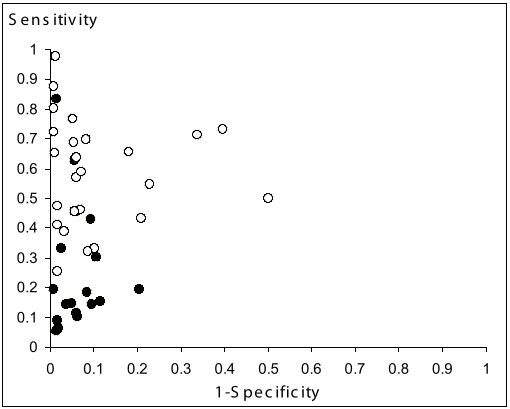
\includegraphics[keepaspectratio]{images/subg.png}}

}

\caption{\label{fig-dtasub}}

\end{figure}%

HSROC and bivariate models can be used to assess heterogeneity by
including covariates. These models allow investigation of the effect of
covariates on sensitivity and specificity separately, rather than just
the DOR (although this can still be obtained).

Different methods can be used to explore heterogeneity in systematic
reviews of diagnostic test accuracy. It should be noted that, as for
meta-regression analyses of other study designs, these analyses are
exploratory, can only include covariates reported by the studies, and
should not be conducted if there are only a small number of studies (a
minimum of 10 studies per covariate is needed). Regardless of the
approach used, study-level factors to be examined should be defined in
the protocol and aspects of methodological quality, (e.g.~QUADAS items)
should be considered individually, rather than as overall quality
scores.

Methods for calculating outcome measures, assessing heterogeneity,
producing plots (both with and without summary estimates) and
undertaking exploratory analyses are available in R. (Team 2025)

\section{Presentation of results}\label{presentation-of-results}

When presenting the results of a systematic review of clinical tests it
is important to consider how these results will be understood by
clinicians and applied in practice.

The presentation of diagnostic measures should be similar for both
narrative and meta-analytic approaches, with graphical representation
and/or tabulation of individual study results and additional results
presented if meta-analysis was performed. Sufficient detail of the
tests, participants, study design and conduct should be presented in
tables.

The 2 x 2 table results of TP, FP, FN and TN together with sensitivity
and specificity, as a minimum should be presented for each study.

The choice of accuracy measures presented depends on the aims and
anticipated users of the review. Sensitivity and specificity and
likelihood ratios are measures of test performance; likelihood ratios
may be more useful in a clinical setting as they can be used to
calculate the probability of disease given a particular test result,
whereas DORs are difficult to interpret clinically.

Forest plots or ROC space plots provide useful visual summaries and can
be easier to interpret than large tables of numbers. The ranges should
be presented when summarizing results which have not been subject to
meta-analytic pooling. For paired results it may be useful to also
present the corresponding measure for the studies at each end of the
range, e.g.~`sensitivity ranged from 48\% (at a specificity of 80\%) to
92\% (at a specificity of 70\%)'.

If a meta-analysis was undertaken then the presentation of results
depends on the methods used. If sensitivity or specificity have been
pooled as individual measures then the summary estimate together with
the 95\% confidence intervals should be presented.

If an SROC model has been used then the relevant SROC curve(s) should be
presented. Where the performance of a number of index tests is being
compared it may be useful to present multiple SROC curves (or un-pooled
data sets) on the same plot. Summary measures of overall diagnostic
accuracy, such as AUC or the Q* point (the point on the curve where
sensitivity and specificity are equal) may also be presented. However,
the relevance of the Q* point is debatable, as its use may lead to
summary estimates of sensitivity and specificity outside the values in
the original studies. Pairs of sensitivity and specificity values can
also be read from the SROC curve and presented as a number of summary
points in order to provide an overall description of the curve. The
estimated SROC curves should also be presented if HSROC or bivariate
models have been used. These models enable the calculation of summary
estimates of sensitivity and specificity, which should be reported along
with their 95\% confidence intervals. Although the use of HSROC or
bivariate models to generate summary likelihood ratios is not
recommended, where likelihood ratios are considered helpful to
interpretation, summary likelihood ratios can be calculated from the
pooled estimates of sensitivity and specificity generated by these
models. For results from a HSROC or bivariate model, as these retain the
paired nature of sensitivity and specificity, a region can be plotted
around the summary operating point which represents the 95\% confidence
intervals of both measures. Confidence interval regions can also be
plotted for the results of individual studies, but care is required to
ensure that these are not mistakenly interpreted as representations of
study weighting. Both models can also be used to plot a prediction
region; this is the region which has a particular probability of
including the true sensitivity and specificity of a future study.

\section{Report writing}\label{report-writing-1}

Systematic reviews of diagnostic test accuracy (DTA) studies are
fundamental to the decision making process in evidence based medicine.
Although such studies are regarded as high level evidence, these reviews
are not always reported completely and transparently. Suboptimal
reporting of DTA systematic reviews compromises their validity and
generalisability, and subsequently their value to key stakeholders. An
extension of the PRISMA (preferred reporting items for systematic review
and meta-analysis) statement must be folllowed to improve the reporting
quality of DTA systematic reviews. (McInnes et al. 2018) The PRISMA-DTA
statement has 27 items, of which eight are unmodified from the original
PRISMA statement.

\textbf{Summary: Diagnostic studies}

\begin{itemize}
\item
  Researchers planning systematic reviews of test accuracy should give
  careful consideration to context.
\item
  Diagnostic tests should be evaluated in patients who are
  representative of those in whom the test will be used in practice;
  ideally a consecutive or randomly selected series whose diagnosis is
  unknown at the time of testing.
\item
  Careful consideration should be given to what is the appropriate
  reference standard to establish diagnosis.
\item
  Difficulties in searching bibliographic databases for test accuracy
  studies and the lack of suitable methodological search filters mean
  that more specific searches carry a risk of missing studies. Searches
  based upon index test and target condition, which are designed to
  maximize sensitivity, are therefore recommended.
\item
  Test accuracy studies are often poorly reported, hampering data
  extraction, quality assessment and synthesis.
\item
  Though often unable to provide a definitive estimate of test accuracy,
  systematic reviews can highlight important gaps in the evidence base
  and aid in the design of future studies.
\end{itemize}

\bookmarksetup{startatroot}

\chapter*{References}\label{references}
\addcontentsline{toc}{chapter}{References}

\markboth{References}{References}

\phantomsection\label{refs}
\begin{CSLReferences}{1}{1}
\bibitem[\citeproctext]{ref-mada}
Doebler P. Mada: Meta-analysis of diagnostic accuracy. 2025; Available
from: \url{https://CRAN.R-project.org/package=mada}

\bibitem[\citeproctext]{ref-GRADEproGDT}
GRADEpro. GDT: Guideline development tool {[}software{]} {[}Internet{]}.
{McMaster University and Evidence Prime}; 2025. Available from:
\url{https://gdt.gradepro.org/app/}

\bibitem[\citeproctext]{ref-higgins2023chapter8}
Higgins JPT, Deeks JJ, Chandler J, Page MJ, Bossuyt PC, Li T, et al.
Chapter 8: Assessing risk of bias in a randomized trial. In: Higgins
JPT, Thomas J, Chandler J, Cumpston M, Li T, Page MJ, et al., editors.
Cochrane handbook for systematic reviews of interventions
{[}Internet{]}. version 6.5 (updated February 2023). Chichester, UK:
Wiley-Blackwell; 2023. Available from:
\url{https://www.cochrane.org/authors/handbooks-and-manuals/handbook/current/chapter-08}

\bibitem[\citeproctext]{ref-ICMJE}
ICMJE. International committee of medical journal editors:
Recommendations for scholarly work in medical journals {[}Internet{]}.
2025. Available from: \url{https://www.icmje.org/recommendations/}

\bibitem[\citeproctext]{ref-McInnes2018}
McInnes MDF, Moher D, Thombs BD, McGrath TA, Bossuyt PM, Clifford T, et
al. Preferred Reporting Items for a Systematic Review and Meta-analysis
of Diagnostic Test Accuracy Studies. JAMA {[}Internet{]}. 2018 Jan
23;319(4):388. Available from:
\url{http://dx.doi.org/10.1001/jama.2017.19163}

\bibitem[\citeproctext]{ref-Moher2015}
Moher D, Shamseer L, Clarke M, Ghersi D, Liberati A, Petticrew M, et al.
Preferred reporting items for systematic review and meta-analysis
protocols (PRISMA-P) 2015 statement. Systematic Reviews {[}Internet{]}.
2015 Jan 1;4(1). Available from:
\url{http://dx.doi.org/10.1186/2046-4053-4-1}

\bibitem[\citeproctext]{ref-Moses1993}
Moses LE, Shapiro D, Littenberg B. Combining independent studies of a
diagnostic test into a summary roc curve: Data{-}analytic approaches and
some additional considerations. Statistics in Medicine {[}Internet{]}.
1993 Jul 30;12(14):1293--316. Available from:
\url{http://dx.doi.org/10.1002/sim.4780121403}

\bibitem[\citeproctext]{ref-grade_2024}
Neumann I, Schünemann H. {The GRADE Book} {[}Internet{]}. version 1.0
(updated September 2024)). The GRADE Working Group; 2024 {[}cited 2025
Oct 6{]}. Available from: \url{\%7Bhttps://book.gradepro.org\%7D}

\bibitem[\citeproctext]{ref-page2021}
Page MJ, McKenzie JE, Bossuyt PM, Boutron I, Hoffmann TC, Mulrow CD, et
al. The PRISMA 2020 statement: an updated guideline for reporting
systematic reviews. Systematic Reviews {[}Internet{]}. 2021 Mar
29;10(1). Available from:
\url{http://dx.doi.org/10.1186/s13643-021-01626-4}

\bibitem[\citeproctext]{ref-Reitsma2005}
Reitsma JB, Glas AS, Rutjes AWS, Scholten RJPM, Bossuyt PM, Zwinderman
AH. Bivariate analysis of sensitivity and specificity produces
informative summary measures in diagnostic reviews. Journal of Clinical
Epidemiology {[}Internet{]}. 2005 Oct;58(10):982--90. Available from:
\url{http://dx.doi.org/10.1016/j.jclinepi.2005.02.022}

\bibitem[\citeproctext]{ref-Rutter2001}
Rutter CM, Gatsonis CA. A hierarchical regression approach to
meta{-}analysis of diagnostic test accuracy evaluations. Statistics in
Medicine {[}Internet{]}. 2001 Sep 5;20(19):2865--84. Available from:
\url{http://dx.doi.org/10.1002/sim.942}

\bibitem[\citeproctext]{ref-sterne2019}
Sterne JAC, Savović J, Page MJ, Elbers RG, Blencowe NS, Boutron I, et
al. RoB 2: a revised tool for assessing risk of bias in randomised
trials. BMJ {[}Internet{]}. 2019 Aug 28;l4898. Available from:
\url{http://dx.doi.org/10.1136/bmj.l4898}

\bibitem[\citeproctext]{ref-base}
Team RC. R: A language and environment for statistical computing. 2025;
Available from: \url{https://www.R-project.org/}

\bibitem[\citeproctext]{ref-Whiting2011}
Whiting PF, Rutjes AWS, Westwood ME, Mallett S, Deeks JJ, Reitsma JB, et
al. QUADAS-2: A Revised Tool for the Quality Assessment of Diagnostic
Accuracy Studies. Annals of Internal Medicine {[}Internet{]}. 2011 Oct
18;155(8):529--36. Available from:
\url{http://dx.doi.org/10.7326/0003-4819-155-8-201110180-00009}

\end{CSLReferences}




\end{document}
